%%% dissertation.tex
%%% no more needs to be said
%
% Alex Barnett, Sept 200%
% Taken from Adam Lupu-Sax and edited May 2000.

% my preferred settings:
% \documentclass[11pt,twoside,final]{huthesis}

% Harvar GSAS Jan 2000 settings:
% (Lauren Lamir 5-1519 gave 12pt Times New Roman as the ideal size).
\documentclass[a4paper,12pt,twoside,final,epsbox,kcite,here]{huthesis}
\usepackage{epsfig,bm,epsf,float}
%\UseTblrLibrary{booktabs}
\usepackage{multirow}
\usepackage{tabto}
\usepackage{float}
\usepackage{booktabs}
\usepackage{nth}
\usepackage{url}
% \usepackage[colorlinks,
%             linkcolor=blue,       
%             anchorcolor=blue,  
%             citecolor=blue,    
%             ]{hyperref}
\newcommand {\R}{\mathbb{R}}
\usepackage{caption} 
\captionsetup[table]{skip=8pt}
\usepackage{array}
\usepackage{xcolor}
\usepackage{color, colortbl}   

\definecolor{Gray}{gray}{0.9}
\definecolor{LightCyan}{rgb}{0.88,0.95,1}

%Equal Margin
%\documentclass[a4paper,12pt,final,epsbox,kcite,here]{huthesis}
%\usepackage{epsfig,bm,epsf,float}
%\addtolength{\oddsidemargin}{-.925cm}
%\addtolength{\evensidemargin}{-.925cm}
% \usepackage{url}
%% choose which files to process
%% stolen from the mitthesis suite

%\typein [\files]{Enter file names to process, (frontmatter,intro,...),
%or `all' to process all files:} \def\all{all} \ifx\files\all
%\typeout{Including all files.} \else \typeout{Including only \files.}
%\includeonly{\files} 
%\fi

% Table of contents max depth listed:
% 1 = section, 2 = subsection, 3 = subsubsection
% (Adam Lupu-Sax had 1. Is this standard at Harvard? I'm going for 2)
\setcounter{tocdepth}{2}

%%%%%%%%%%%%%%%%%%%% nammoto %%%%%%%%%%%%%%%%%%%%
\usepackage[tight]{subfigure}
\usepackage{afterpage}
\usepackage{multirow}
\usepackage{emptypage}

%\newcommand{\argmax}{\mathop{\rm arg~max}\limits}
%\newcommand{\argmin}{\mathop{\rm arg~min}\limits}

%%%%%%%%-----Kingkan-------%%%%%%%%%%%%%%
\usepackage{CJKutf8}  % Japanese font
\usepackage[T1]{fontenc} 
\usepackage[utf8]{inputenc}
\usepackage{amsmath}
\usepackage{amssymb}

%%%%%%%%%%%%%% Ford %%%%%%%%%%%%%%
%\usepackage[hyphens,spaces,obeyspaces]{url} %%%% use either this or hyperref and don't forget to \url{} in .bib
% \usepackage{hyperref}

% we also can use this
\usepackage[hyphenbreaks]{breakurl}
% \Urlmuskip=0mu plus 4mu
%%%%% above packages are loaded in order, this is done to fix weird spacing in bib. 
\usepackage[section]{placeins}
\usepackage{bm}
\usepackage{mathtools}

% \graphicspath{{images/}}
% \setlength{\subfigtopskip}{15pt}
% \setlength{\subfigcapskip}{-10pt}
% \setlength{\subfigbottomskip}{5pt}
% \renewcommand{\arraystretch}{1.5}

%%%%%%%%%%%%%% Wasu %%%%%%%%%%%%%%%%%%%%%%%%%%
% \usepackage{natbib} % for citeyar citeauthor <<- doesnt work, didnt used
\usepackage{amsfonts} % \mathcal , \mathbb
\usepackage{amsmath} % \subset
\usepackage{bbm} % \mathbbm for number 1 bb
% \usepackage{caption}
\usepackage{subcaption}
\usepackage{tabularx}
\usepackage{listings}

\lstdefinelanguage{json}{
    basicstyle=\normalfont\ttfamily,
    numbers=left,
    numberstyle=\scriptsize,
    stepnumber=1,
    numbersep=8pt,
    showstringspaces=false,
    breaklines=true,
    frame=lines,
}

%%%%%%%%%%%%%%%%%%%% the text of this dissertation %%%%%%%%%%%%%%%%%%%%

\begin{document}

%\input{mathdefs} % my math definitions.

% UNDERLYING SPACING FOR WHOLE DOCUMENT:
% Single spacing: takes place of `draft' mode, without losing figures.
% \ssp

% makes double-spaced: (for GSAS requirement, microfiche):
\dsp

%%%%% frontmatter %%%%%%%%%%%%%%%%%%%%%
%\cleardoublepage
%\thispagestyle{plain}

%frontmatter.tex
\title{Discovering Improved Feature Spaces for Unsupervised Visual Anomaly Detection for Industrial Products}
\japtitle{(より良いマルチモーダル表現の学習を通じた医療視覚質問応答の性能向上)}
\author{Mukhammad RAKHIMOV Shukhrat Ugli}
\degreemonth{February}  %month final submission occurs. 
\degreeday{6} 
\degreeyear{2025}
\degree{Master} 
\department{System Information Sciences} 
\field{Information Sciences} 
\advisor{Prof. Takayuki OKATANI}
\maketitle
\clearpage\null{\thispagestyle{empty}}
%%%%%%%%%%%%%%% Abstract %%%%%%%%%%%%%%%
%\pagenumbering{roman}
%\setcounter{page}{-4}
 %% Abstract.tex

%%%%%%%%%%%%%%% Abstract %%%%%%%%%%%%%%%

\cleardoublepage
\begin{abstract}
%\renewcommand{\baselinestretch}{1.2}\normalsize
\renewcommand{\baselinestretch}{1.2}\abstractfont

Computer vision models have been instrumental in detection of anomalies in industrial manufacturing processes. Automation of the detection of anomalies plays a crucial role in reducing the production cost while maintaining quality control and ensuring the consistency and reliability of production lines. Current models are capable of categorizing the products as anomalous or nominal, moreover the models can outline the defective region with high accuracy.

% anomaly detection

Contemporary industrial anomaly detection models utilize multiple types of approaches. Three successful methods are: k-nearest neighbor method where statistical outliers are detected on the feature space of a pre-trained network, reconstruction based methods where a decoder is trained to predict the input of an encoder in the form of pre-trained network, student-teacher base methods where a student network is trained to match the output of the teacher pre-trained network.

% problem
As was mentioned, the use of pre-trained networks is prevalent in industrial anomaly detection models. The lack of large industrial datasets and the scarcity of samples with anomalies in those datasets make the use of classical learning methods impractical. Therefore, in the recent year, there has been an emergence of industrial anomaly detection models that rely on the features extracted by pre-trained neural networks. Out of all available pre-trained models for use as a backbone in industrial anomaly detection models, models trained on the ImageNet1k classification task are the dominant choice. ImageNet1k is a general-purpose dataset that consists of 1,000 different classes of 1,281,167 training images. While the usage of ImageNet1k-trained backbones is the dominant idea and has been shown to be effective in most cases, this thesis proposes that training on ImageNet1k generates feature spaces that are general purpose, and better performance of industrial anomaly detection models could be achieved with more specialized feature spaces generated by various methods. This investigation aims to explore and validate these alternative feature spaces to enhance model performance in detecting industrial anomalies.

% method
In this thesis we explore methods of forming specialized feature spaces for industrial anomaly models with the purpose of improving their performance. The main proposal of this thesis is to investigate if a dataset can be formed such that, features extracted from such a dataset would show an improvement in the accuracy of anomaly detection models. The proposed method is to extract a subset of images from a large image dataset such as Laion5b, Laion400m, YFCC100M etc. while ensuring the relevancy of the images that are being extracted to the industrial use cases. To achieve that task, we train an "extractor" bi-class(which are industrial and non-industrial) classifier model, and apply the extractor model to the large image dataset. To train the "extractor" model we form another dataset that contains images consisting of industrial and non-industrial classes.

% check other backbones
In addition to the generation of an industrial-specialized dataset, this thesis explores the effect of other feature spaces that have not been widely utilized in industrial anomaly detection models. Specifically, during our experiments, it was discovered that Vision Transformer-based models as backbones tend to perform considerably worse compared to CNN-based models. This observation highlights the limitations of Vision Transformer models in capturing the intricate patterns and features necessary for effective anomaly detection in industrial settings. Furthermore, out of all available CNN-based models, ResNet-based models showed superior performance, demonstrating their robustness and effectiveness in this domain. More precisely, WideResNet50 and WideResNet101 models proved to achieve the highest accuracy when used as backbones for industrial anomaly detection models.

% Evaluation
To evaluate the performance of different pre-trained models as backbones, we test them using with different types of industrial anomaly detection models. Throughout all the experiments we use MVTechAD dataset, which contains over 5000 images of industrial objects consisting of 15 different categories. For the experiments of this thesis we use PatchCore as it is one of the most common IAD models. 

%First exp
To train the "extractor" models we set up a dataset consisting of 2 classes, industrial and non-industrial. Main part of the dataset consist of ImageNet1k classes manually separated into two categories. We train our extractor ResNet50 on the constructed dataset with the classification task. The resulting extractor model then used to extract industrial class images from a large image dataset, in our case YFCC100M. This results in a unlabeled dataset consisting of more that 2 million images. Due to the unlabeled nature of the generated dataset, we use self-supervised learning methods to achieve feature extraction.  

%Second exp
Although it is common for Vision Transformer models to be used self-supervised learning, experiments showed that, using ViT models as backbones are ineffective compared to CNN models. Therefore, we train WideResNet50 using DINO self-supervised learning pipeline on the dataset formed from applying the extractor model on the YFCC100M dataset. We perform self-supervised learning with the same conditions on the randomly extracted dataset. Three WideResNet50 models are compared using as backbones to two industrial anomaly detection model PatchCore.

% Conclusion
In conclusion, this thesis demonstrates that the choice of feature space and backbone architecture significantly impacts the performance of industrial anomaly detection models. By generating a specialized dataset and exploring alternative feature extraction methods, we have shown that more tailored feature spaces can enhance detection accuracy. However, ImageNet pre-trained feature extractors proved to be surprisingly fit for industrial anomaly detection tasks. Our experiments confirmed the superiority of CNN-based models, particularly WideResNet50 and WideResNet101, over Vision Transformer models. The findings highlight the potential of self-supervised learning on industrial-specific datasets to further improve anomaly detection capabilities. Future research should continue to refine these approaches, potentially leading to more robust and efficient industrial anomaly detection systems.

%---Put blank line before the "end" command-----%

\end{abstract}
%\clearpage\null{\thispagestyle{empty}}
\thispagestyle{empty}
% \clearpage\null{\thispagestyle{empty}}
%\setcounter{page}{0}
%%%%%%%%%%%%%%% Table of Contents %%%%%%%%%%%%%%%
% \cleardoublepage
\cleardoublepage
% \thispagestyle{empty}
% \mbox{}
% \newpage

\pagenumbering{roman}
\setcounter{page}{1}
\addcontentsline{toc}{section}{Table of Contents}
%\pagenumbering{roman}
% 
%\setcounter{page}{0}
\tableofcontents

%%%%%%%%%%%%%%% List of Figures & Tables %%%%%%%%%%%%%%%
%\cleardoublepage
\listoffigures
% \cleardoublepage
\listoftables
% \clearpage\null{\thispagestyle{empty}}
%%%%%% text %%%%%%%%%%%%%%%%%%%%%%%%%%%%
%
%%% Chapter 1
\cleardoublepage
\pagenumbering{arabic}
\setcounter{page}{1}
\chapter{Introduction}
\label{chapter:intro}

%iad_field
In our modern times when we strive to automate every menial task that was resolved by human labor, one of the fields that have been the most important is the industrial manufacturing processes. In improving the process of production, the key point is to ensure the reliability of the process and the quality of the produce. Throughout the recent years, the use of Machine Learning algorithms, specifically Computer Vision models, have showed to be a powerful tool in detecting the defects(called anomalies in the field of machine learning). Therefore, a new field: Industrial Anomaly Detection was formed, which focuses on researching and developing efficient computer vision models in the field. There are generally two types of architectures in the industrial anomaly detection models: feature embedding based architectures and reconstruction based architectures. Most contemporary models are trained without supervision and they, due to the lack of large scale image dataset of industrial objects and the unbalanced nature of available datasets towards nominal samples, rely on the feature space of a pre-trained model.

%iad_arch
The training process depends on the architecture of the model. In feature-embedding types of architectures, usually the training process involves performing a feature extractions and saving them with various modifications. Thereafter, during inference same feature extraction applied to the image being inferred followed by various statistical methods used to calculate the anomaly score of the sample. An example for the feature embedding architecture can be a model PatchCore, which saves nominal features in the memory bank after applying neighborhood aggregation and utilized k-nearest neighbor method to calculate an anomaly score. In reconstruction based methods, autoencoder models is trained either on the features extracted by the pre-trained model or the pre-trained model is used as an encoder inside the autoencoder. For example, in the RealNet model multiple autoencoders are trained on the layers of the feature extractor model. 

\begin{figure}[h]
\begin{center}
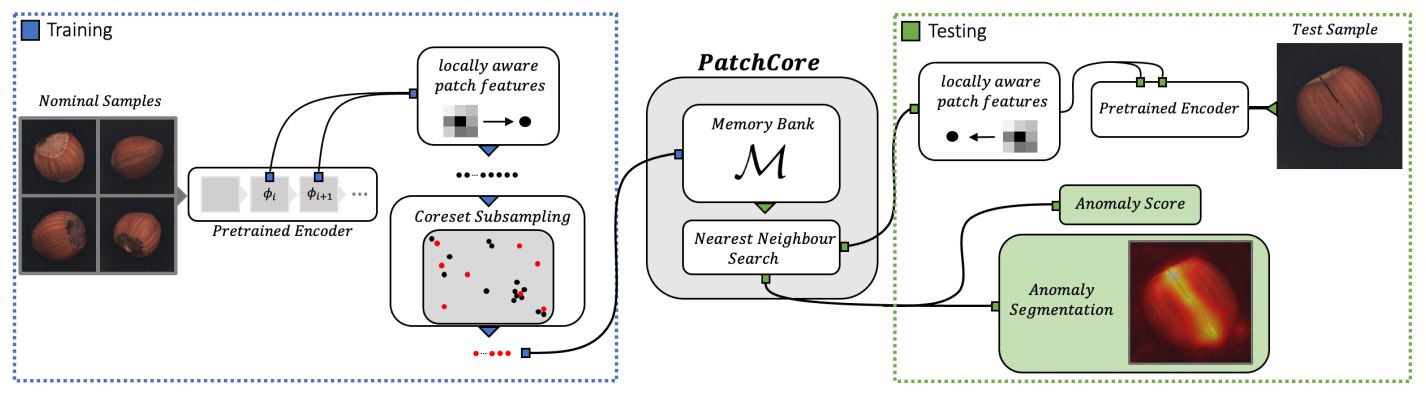
\includegraphics[width=1.0\linewidth]{Chapter_1/patchcore.png}
\end{center}
\caption{Medical Visual Question Answering (VQA) \cite{liu2021slake} is a task where the model receives medical images and corresponding questions as input and produces accurate answers as the output.}
\label{fig:patchcore}
\end{figure}

In this paper we hypothesize that using ImageNet pre-trained models as feature extractors in industrial anomaly detection models can be a potential bottleneck of performance due to the generalized nature of the ImageNet dataset. There is a large representation mismatch between ImageNet which contains a large quantity of natural samples whereas the IAD requires features which represent industrial objects more accurately. Our hypothesis implies that most if not all existing models could benefit from a more specialized feature space which is extracted from datasets with focus on more industrial settings rather than being general or having natural samples.

In order to address this issue the thesis proposes to generate a feature space that would represent the type of data that is used in industrial anomaly detection tasks. In order to accomplish this task, we propose extracting an industrial setting sub-datasets from a large multi-purpose dataset, followed by performing a training on the extracted dataset to have a feature extractor. Throughout this process it is important to choose appropriate dataset to extract from, a proper self supervised learning method and an accurate extraction method. All three parts of the pipeline are important and have to be a deliberate choice, however the most important part and the defining factor for the quality of the extracted features is the extraction method.

In this thesis we opted to utilize a ResNet50 model trained on the dataset curated by hand. However, in this thesis, we will also be discussing other possible options for industrial image extractors. Due to the unlabeled nature of the extracted dataset by the method of our choice, this work will use the DINO unsupervised learning method on all experiments as a feature learning tool. The choice is also motivated by the capability of DINO to train both Vision Transformer and Convolution based networks.

To evaluate the accuracy of different feature spaces against each other, we use PatchCore as the main industrial anomaly detection model. All pre-trained models are to be used as backbones for the model and evaluated on the accuracy of the model on MVTechAD dataset. Firstly, we perform experiments on ViT based backbones because Vision Transformers are more robust for self-supervised learning method which we utilize in this work. However, with further experiments we show that convolution based models are much better fit for the task of industrial anomaly detection. And lastly we provide comparisons between random extraction of images, selective extraction of images and state-of-the-art backbone when used with PatchCore model.

This chapter serves as the introduction to the thesis, offering a comprehensive overview of the research topic and highlighting its significance within the field. Chapter~\ref{chapter:ch2} will focus on the Related Work, delving into the concept of visual question answering, Transformer attention models, and examining recent advancements in vision-language pre-training techniques that have demonstrated effectiveness in addressing various medical vision-language tasks. Chapter~\ref{chapter:ch3} will address the limitations of previous work and introduce the proposed method as a solution. It will highlight the key improvements and contributions of the proposed two-stage pre-training method. In Chapter~\ref{chapter:ch4}, we will conduct a series of comprehensive experiments to evaluate the proposed method. This chapter will provide detailed information about the experimental setup and methodology used. Additionally, it will include an in-depth analysis of the obtained results, demonstrating the performance of the proposed method and its effectiveness in addressing the medical visual question answering. In Chapter~\ref{chapter:ch5}, we will summarize the key findings obtained from our research and provide a comprehensive conclusion. We will also discuss potential areas for further improvement and future research directions in the field, aiming to contribute to the advancement of knowledge and advancements in the topic.

In this introductory chapter we unveiled the field of Industrial Anomaly detection and the potential accuracy bottleneck present in most applications. In the Chapter~\ref{chapter:ch2} the Related Work will be thoroughly discussed, namely the topics will be Vision Transformers, Residual Networks, Wide Residual Networks and their architectural differences. Moreover, we will further discuss PatchCore and RealNet models and their use of pre-trained networks. Chapter~\ref{chapter:ch3} will focus on the possible bottleneck of using ImageNet pre-trained networks as feature extractors and the solutions that can be engaged to address the issue. Chapter~\ref{chapter:ch4} contains the demonstration of the potential of the proposed solution through empirical evidence, conducted series of experiments will be explained in detail. And lastly, Chapter~\ref{chapter:ch5} will serve as a conclusion where we will summarize the results of this work. Moreover, it the last chapter, we will suggest multiple methods of feature space generation that can be explored in further research.

%%% Chapter 2
% \clearpage
% \thispagestyle{empty}
% \mbox{}
% \newpage
\cleardoublepage
\chapter{Related Work}
\label{chapter:ch2}
In this chapter we will thoroughly discuss works related to the current thesis. Firstly we explore computer vision model architectures that are used as feature extractors, namely Vision Transformers, Convolutional Neural Networks, Residual Networks and Wide Residual Networks. We will investigate the differences between aforementioned architectures in order to bring attention to their drastic difference in performance as feature extractors for industrial anomaly detection models. Second, we will delve into the topic of unsupervised and self-supervised learning specifically. The comprehensive analysis of self-supervised learning model DINO, which we utilize broadly in this work due to the unlabeled nature of a dataset extracted with our method, will be provided. Thereafter, a detailed discussion on Industrial Anomaly Detection will be provided. This section will also present the challenges the field faces with the scarcity of diverse training data and the need of Unsupervised Industrial Anomaly Detection models. Lastly, we will study the architecture of two industrial anomaly detection models used in the experiments present in this work. The first model we analyze is PatchCore models which uses saves extracted features in a memory bank. And the second model is RealNet which trains auto-encoders on the layers of feature extractor model.

\section{Vision Transformer}
\label{vit}
Introduction of Vision Transformers have presented a significantly different approach to computer vision tasks, where the standard approach of using convolutional neural networks have been replaced by transformer architecture. Until the point of introduction of vision transformers, transformer architecture was commonly used for natural language processing tasks. Transformer architecture leverages self-attention mechanism which has the ability to capture relationship between all parts of data with each other. In case of Vision Transformers, self-attention mechanism is able to capture the global context of the image rather than focusing on local features as CNN filters do.

One of the main challenges when it comes to utilizing transformer architecture on visual data, is that it does not have the ability to capture spatial information as the traditional CNN models do. Moreover, transformers are originally equipped to work with sequential data like a stream of words which images are not. In order to make images a viable input for transformer, the image is split into constant size patches which are then embedded with positional encodings saving crucial spatial information. Transformer evaluates the relationships between all the patches using the self-attention mechanism. Thereafter, output from the transformer is used as an input for classification feed-forward network. In the case of Industrial Anomaly Detection, output from each transformer layer can be used as extracted features in anomaly detection models. The diagram of the ViT architecture is shown on the figure \ref{fig:vit}.

\begin{figure}[h]
	\begin{center}
		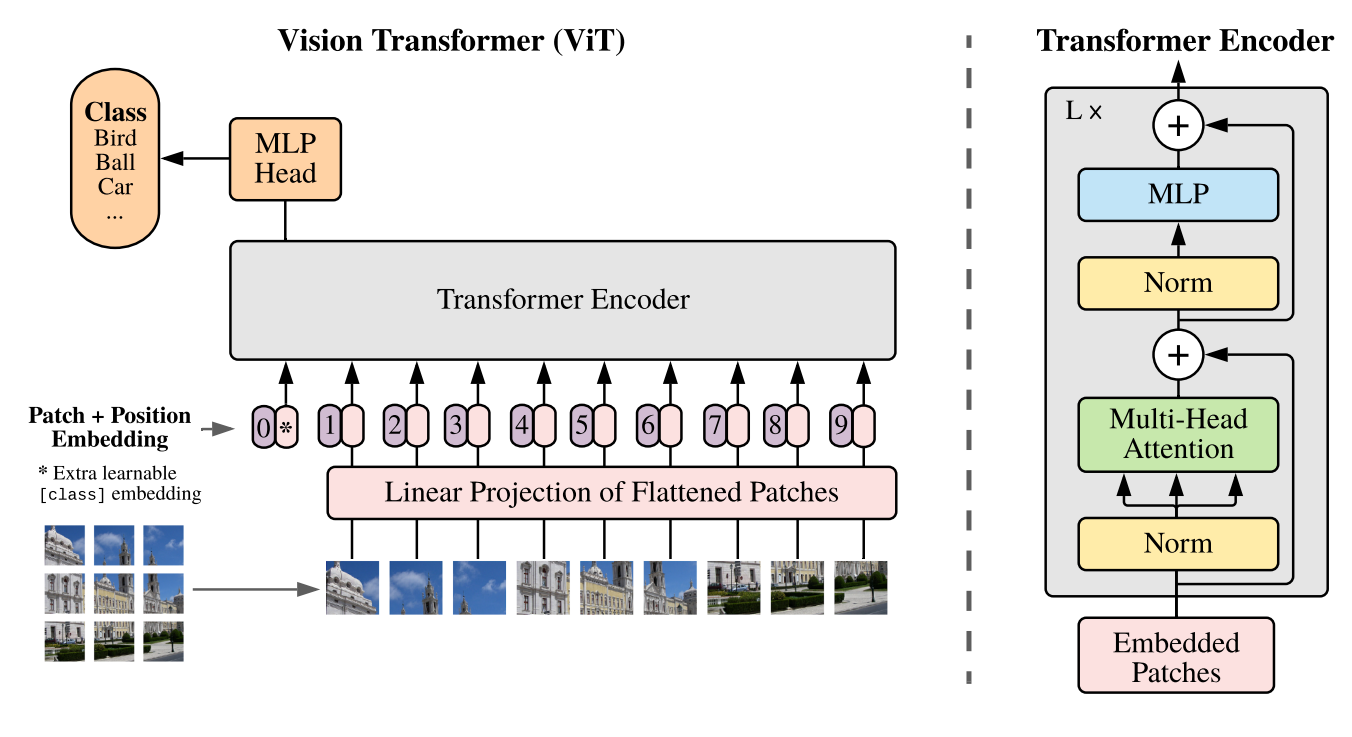
\includegraphics[width=0.8\linewidth]{Chapter_2/vit.png}
	\end{center}
	\caption{Vision Transformer model which uses the Transformer encoder shown on the right to capture meaningful features from the images. The images have to be split into patches to transform them into a sequential data in order to make them to be able to be captured by Transformers.}
	\label{fig:vit}
\end{figure}

In the recent years Vision Transformers have been used extensively in self-supervised learning models. The prevalence of Vision Transformers in self-supervised learning can be explained by the ability of them to utilize the global context of images, which allows them to be able to extract high quality features from unlabeled data. Methods like contrasive learning proved to be very efficient when used in combination with Vision Transformers especially.

\section{Convolutional Neural Networks}
\label{cnn}
For many years Convolutional Neural Networks have been the main architecture in the field of image processing due to their ability to capture spatial hierarchical features. They have been used efficiently in tasks such as image classification, semantic segmentation and object detection. When this architecture was introduced by Yann LeCunn and colleagues in 1980, it revolutionized the field showing significant increase in accuracy over the methods that used to be prevalent.

The main novelty that Convolutional Neural Networks introduced were the convolutional and pooling layers of the network. Convolutional layer performs a "convolution" operation using kernels on the input image or, in the later layers, on the features extracted by the filters of the previous layer. In the first layers, local features are captured by convolution and in the later layers, pooling operation is performed, which serves as dimensionality reduction and extraction of global features from local ones. In more recent models convolution and pooling layers are also followed by normalization layers, which stabilizes and speeds up the training process. Between each layers of the model, some non-linearity function, which is usually ReLU activation function, is used to allow the model to learn to generalize more complex structures of data. Generally, the final stage of CNN architectures consist of fully-connected layers that maps the learned features to specific classes. To have a better understanding of the architecture please look at the figure \ref{fig:cnn}

\begin{figure}[h]
	\begin{center}
		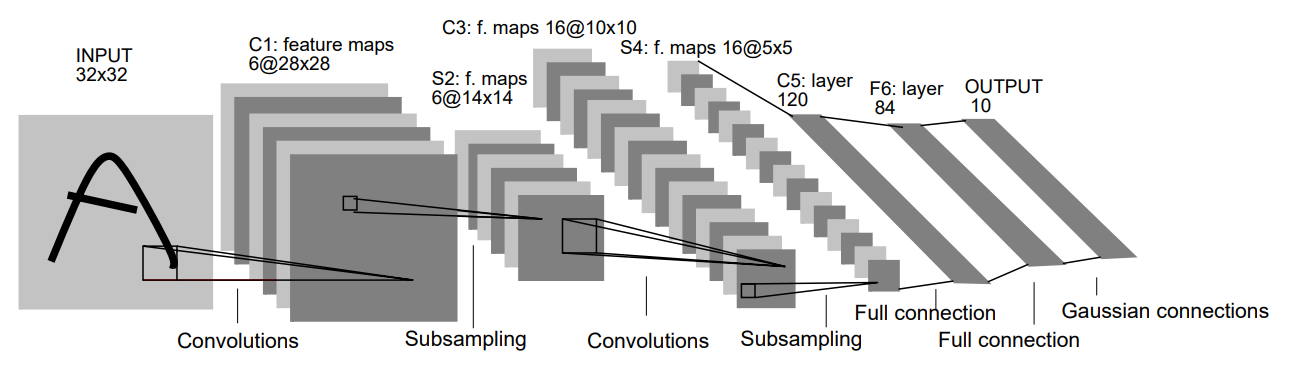
\includegraphics[width=1.0\linewidth]{Chapter_2/cnn.png}
	\end{center}
	\caption{Convolutional Neural Network consisting of convolution and subsampling layers. Its architecture allows for the efficient capture of spatial features, which can explain its prominence in anomaly detection models.}
	\label{fig:cnn}
\end{figure}

In spite of the fact that Vision Transformers have been emerging as the competitor to the CNN architectures, CNN architectures still stand as the preferable option in certain specific cases, Industrial Anomaly Detection being one of them. The ability of CNNs to capture local features and spatial hierarchies with high accuracy, can contribute to their efficiency as feature extractors in IAD models.

\subsection{Residual Networks}
\label{resnet}
Residual Network architectures are the subset of CNNs that are designed for deep learning scenarios and address one of the main challenges of training deep neural networks. The architecture presented a concept of skip connections which is a connection between layers that skips some layers(usually one) in between. This new addition allows models to have hundreds of layers, which was impossible due to the vanishing gradients problem.

The usual ResNet model consists of residual blocks that have a skip connection at the input connecting directly to the output of the block. Skip connection(figure \ref{fig:res_block}) facilitates the model to learn a residual mapping F(x) = H(x) - x, instead of the direct H(x) mapping from the input x, which allows the model to learn residuals or differences, rather than the one-to-one mapping. Each residual block contains multiple convolutional layers and activation layers. In most of the ResNet implementations, such as ResNet50, a bottleneck residual connection is used which consists of a 3x3 convolution layers in between two 1x1 convolution layers. All the innovation present in ResNet architecture allows for the training of multi layer deep models without the vanishing gradients problem and preserving the learned features across layers.

\begin{figure}[h]
	\begin{center}
		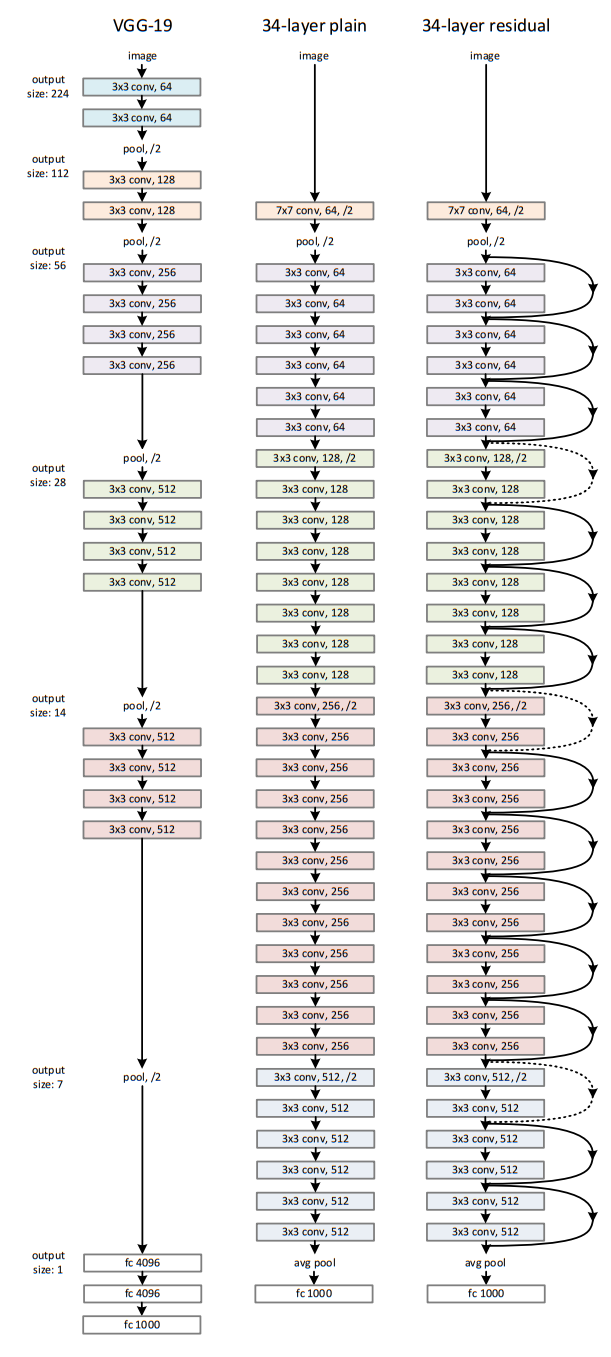
\includegraphics[width=0.5\linewidth]{Chapter_2/resnet.png}
	\end{center}
	\caption{Residual block that allows for the assembly of deep computer vision models.}
	\label{fig:res_block}
\end{figure}

Residual Networks emerged as a dominant model to be used as feature extractors in industrial anomaly detection models. This choice is driven mainly by empirical evidence to their efficiency. However, we can also see that in ResNet models the advantages of CNNs, such as capturing local features and spatial hierarchies, are amplified by allowing us to train larger size CNN models. Advantages which might make CNNs a preferable choice as feature extractors for IAD models.

\subsection{Wide Residual Neural Networks}
\label{wideresnet}
Wide Residual Networks are enhancement upon the regular ResNet architecture, which focus on increasing the width of the model instead of the depth. The main point of this improvement is in the residual blocks where the channels of convolutions are increase by some factor(figure \ref{fig:wide_resnet}), allowing the model to have increase representational capacity while maintaining the ability to train deep networks. Increased channel size also allows Wide ResNets to have improved gradient flow which enhances the models capability to learn from large complex datasets. The enhancements allow Wide ResNets to have higher capacity to learn fine-grained details which makes this type of architecture a suitable choice for usage as feature extractors in IAD models.

\begin{figure}[h]
	\begin{center}
		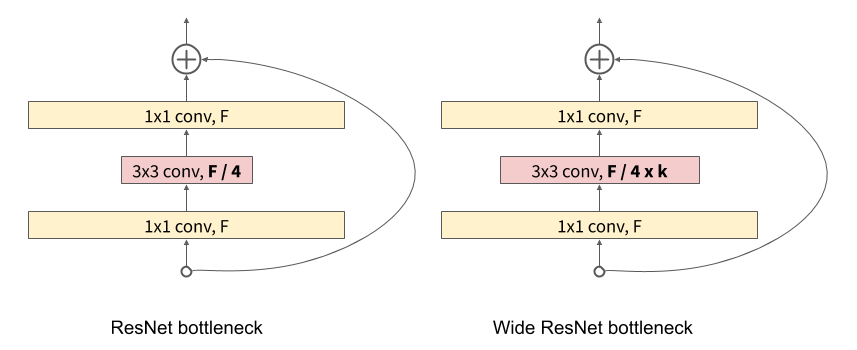
\includegraphics[width=1.0\linewidth]{Chapter_2/wide_resnet.png}
	\end{center}
	\caption{Difference between Wide Residual Block and standard residual block, where the wide residual network has the width increase by the factor of k}
	\label{fig:wide_resnet}
\end{figure}

\section{Unsupervised Learning}
\label{usupervised learning}
To generate feature spaces suitable for industrial anomaly detection tasks, it is beneficial to use multiple available, large scale, unlabeled image datasets. One of the many Unsupervised Learning techniques will allow us to effectively extract features from unlabeled datasets. Unsupervised Learning refers to the variant of machine learning algorithms where the models is trained to learn patterns in the data itself, instead of overt output labels like in supervised learning. Unsupervised Learning models in their process leverage such architectures as autoencoders which work by first transforming the data into a compressed representation and then learning to restore the input, generative adversarial networks which train two competing models discriminator and a generator, clusterization algorithms which separates the input into clusters using algorithms like k-NN, contrasive learning which learns features by comparing input data. 

\subsection{Self-supervised Learning}
\label{self-supervised learning}
Self-supervised learning are a subset of unsupervised learning models in that, they also designed to learn from unlabeled data but unlike unsupervised learning models that learn representation from the data directly, self-supervised learning first assigns "labels" or "tasks" on unlabeled data and learns to fit the generated labels or complete the generated tasks in order to extract hidden structures and patterns from the provided input. Therefore, self-supervised learning serves as the middle ground between unsupervised and supervised learning, in an attempt to leverage the advantages of supervised learning in an unsupervised setting. Over the recent years, self-supervised learning models proved to be very efficient method of unsupervised learning, allowing to train models that can perform with high accuracy on multiple tasks after the task specific fine-tuning process.

As have been stated the key component of self-supervised learning is the generation of assisting tasks based on the training data. An example for the types of tasks that might be generated can be, predicting various transformations applied on the image or drawing in the random missing patches of the image. By training to accomplish this tasks, self-supervised model learn the patterns that inherently exist in the data, extracting valuable features in the process. This mode of learning can be utilized to generate feature spaces suitable for the task of industrial anomaly detection from large scale unlabeled datasets. Indeed, we use one of the most robust self-supervised learning models DINO in this work.

\subsection{DINO model}
\label{dino}
DINO(from distillation with no labels) is a robust self-supervised learning model that was introduced by Facebook AI team that uses enhanced knowledge distillation pipeline to learn useful representations from an unlabeled large image datasets. The model achieves high accuracy on top-1 classification task on the ImageNet dataset, specifically 79.1 percent when training the model ViT-S/14 and higher 82.1\% when used with the ViT-B/14 model. DINO models ability to train both Vision Transformer and CNN based model and its high efficiency makes the model an excellent choice for the purposes of this thesis.

In its training process DINO utilizes the teacher-student architecture where student is trained to align its output to the output of the teacher model. Both student and teacher models trained using the same model architecture but using different parameters. The key point of the DINO model is that the teacher model is trained using the EMA - exponential moving average of the student model in order to guarantee the stability during training. Training process itself consists of passing an input image with random transformations picked from a constant set of transformations, to teacher and student models and adjusting the student models output to the teacher models output using cross-entropy loss function. During such a training process, the student model learn invariant and meaningful features from the input. The architecture is shown in the figure \ref{fig:dino}

\begin{figure}[h]
	\begin{center}
		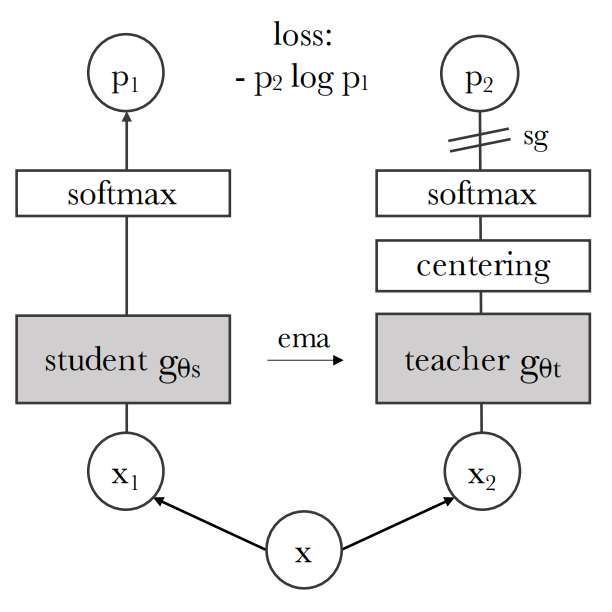
\includegraphics[width=0.5\linewidth]{Chapter_2/dino.png}
	\end{center}
	\caption{architecture of a DINO model consiting of a student and a teacher model.}
	\label{fig:dino}
\end{figure}

\section{Industrial Anomaly Detection}
\label{iad}
Industrial Anomaly Detection has become the irreplaceable part of various manufacturing processes, allowing to detect any deviations from standards of manufacturing and preventing defective products from potentially reaching the output. Anomalies of varying kind expected to happen in every industrial processes due to different reasons like, wear and tear, software errors and malfunction of devices. Industrial Anomaly Detection methods allow us monitor the manufacturing pipeline and to anticipate such defects, followed with swift corrections. This allows for increased stability of manufacturing, improved quality control, mediating costly defects, minimizing downtime and enhancing efficiency. For the visual explanation, refer to \ref{fig:iad}

\begin{figure}[h]
	\begin{center}
		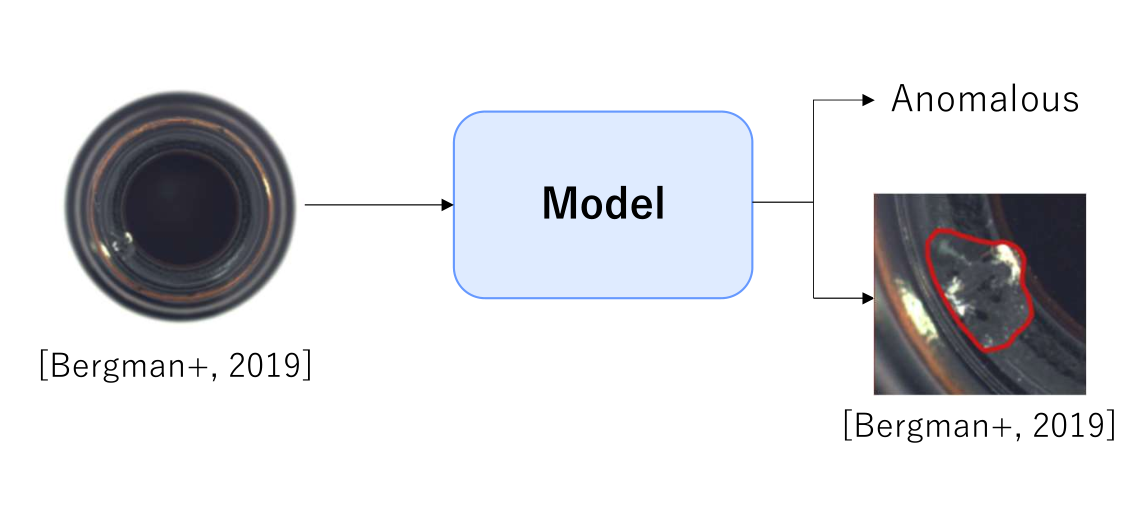
\includegraphics[width=0.8\linewidth]{Chapter_2/iad.png}
	\end{center}
	\caption{The process of Industrail Anomaly Detection}
	\label{fig:iad}
\end{figure}

Contemporary Industrial Anomaly Detection methods heavily rely on deep learning computer vision models. Variety of computer vision models like convolutional neural networks, vision transformers and autoencoders can be utilized to efficiently implement industrial anomaly detection in real use case scenarios where data from visual sensors such as cameras. These models posses the ability to learn complex visual representation from high-dimensional imagery data, allowing IAD tasks to be performed with high accuracy and reliability. Over the recent years the field of Industrail Anomaly Detection witnessed a lot of improvements, especially in the field of Unsupervised Industrial Anomaly Detection where there is a scarcity of anomalous data. 

\clearpage
\subsection{Unsupervised Industrial Anomaly Detection}
\label{unsupervised iad}
Unsupervised Industrial Anomaly Detection leverage unsupervised deep learning techniques in order to learn any deviations from the nominal patterns it the provided input. In IAD field unsupervised learning is vital because labeled anomalous images are extremely scarce or non-existent. There are multiple types of architectures that can be engaged to implement unsupervisded iad models, including architectures like autoencoders, clustering and various statistical techniques are common to be used. As an example, PatchCore model uses memory-bank approach opting to save features extracted by pre-trained backbone model with some aggregation operations while on the inference performing kNN over the saved features and extracted features of the test sample. Another model called SimpleNet trains a discriminator with synthetically generated anomalies on the features of the nominal samples. There are also reconstruction based models like RealNet which utilized auto-encoders on the layers of the pre-trained feature extractor model. In this thesis, we use these three models to test different feature spaces on. Refer to figure \ref{fig:uiad} for the visual representation of the Unsupervised IAD process.

\begin{figure}[h]
	\begin{center}
		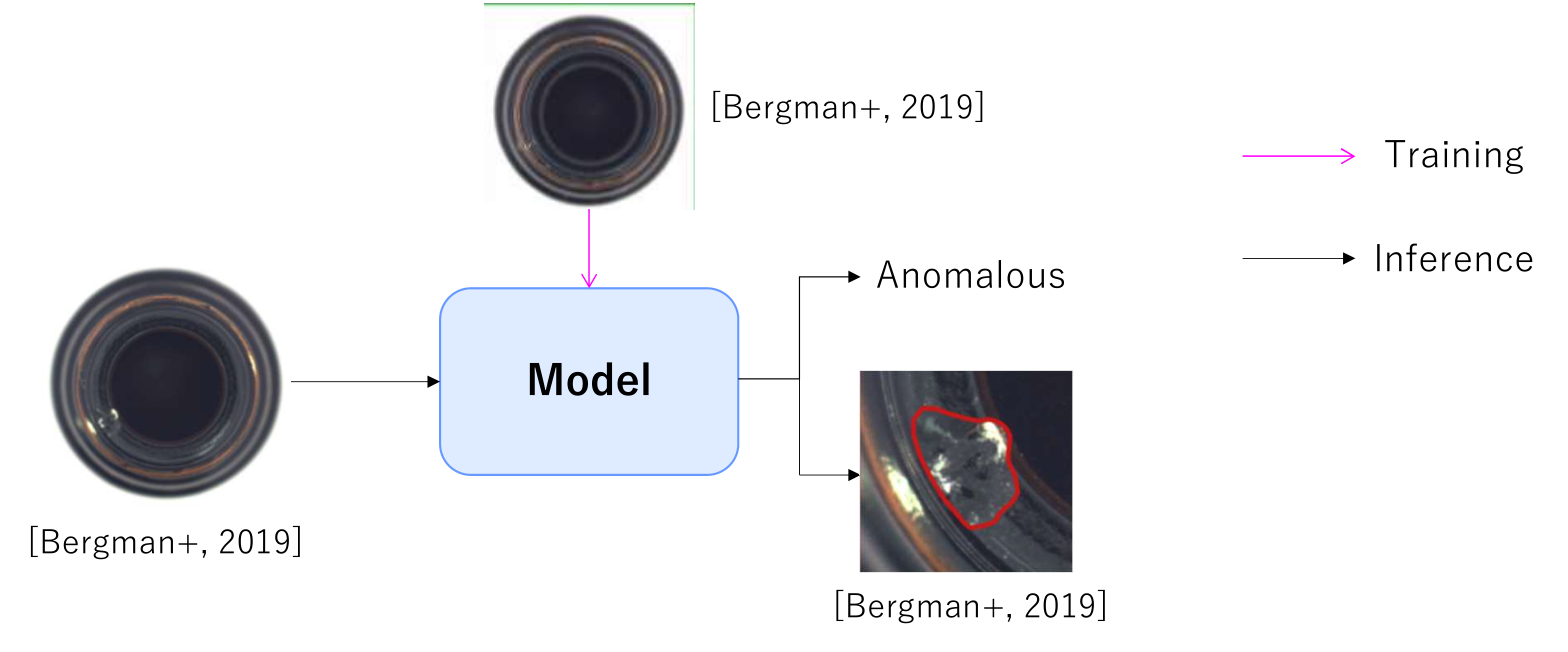
\includegraphics[width=0.8\linewidth]{Chapter_2/uiad.png}
	\end{center}
	\caption{Unsupervised anomaly detection pipeline.}
	\label{fig:uiad}
\end{figure}

\clearpage
\subsection{PatchCore}
\label{patchcore}
The PatchCore industrial detection model is designed to excel in identifying anomalies in visual data for industrial applications. The methodology behind PatchCore involves several key steps. Initially, the model utilizes pre-trained convolutional neural networks (CNNs) to extract high-dimensional feature representations from input images. These features are then divided into smaller patches, which are processed individually. The core idea of PatchCore is to leverage these patches for local anomaly detection, ensuring that even small, subtle defects can be detected. The model applies an anomaly scoring mechanism to each patch, comparing it to a reference distribution of normal patches derived from a training dataset. This scoring helps in distinguishing between normal and anomalous regions within an image. Additionally, PatchCore incorporates a memory bank of normal patches, enabling efficient and accurate comparison during inference. By focusing on local patches rather than the entire image, PatchCore enhances the precision and reliability of anomaly detection, making it well-suited for diverse industrial inspection tasks where fine-grained anomalies are critical to detect.

\section{MVTechAD}
\label{mvtech}
The MVTec Anomaly Detection (MVTec AD) dataset is a comprehensive benchmark specifically designed for evaluating anomaly detection methods in industrial inspection. It comprises over 5,000 high-resolution images across fifteen different object and texture categories, each containing defect-free training images and a test set with various types of defects. The dataset provides pixel-precise annotations of all anomalies, enabling precise evaluation and comparison of different anomaly detection techniques. MVTec AD is widely used in the research community to advance and validate new methods, ensuring they are robust and effective for real-world industrial applications. Samples from the dataset are displayed in the figure \ref{fig:mvtec}.

\begin{figure}[h]
	\begin{center}
		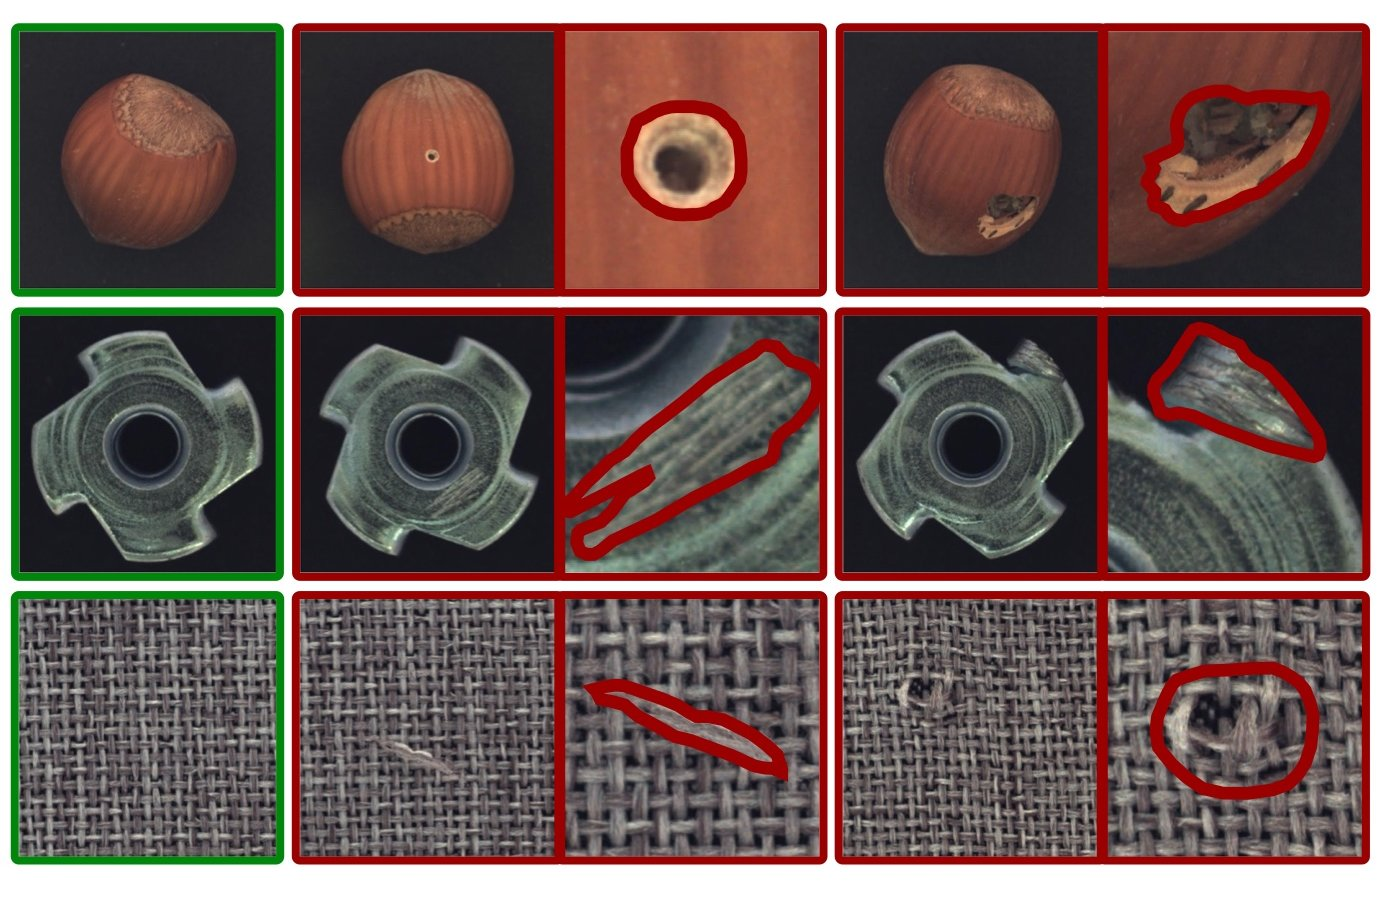
\includegraphics[width=0.7\linewidth]{Chapter_2/mvtec.jpg}
	\end{center}
	\caption{Samples from MVTech dataset.}
	\label{fig:mvtec}
\end{figure}


%%
%%% Chapter 3
\cleardoublepage
% \thispagestyle{empty}
% \mbox{}
% \newpage
\chapter{Addressing Feature Space Shortcomings through Selective Image Extraction}
\label{chapter:ch3}

This chapter will focus on the current state of Industrial Anomaly Detection, namely the use of pre-trained backbones in the unsupervised industrial anomaly detection models. We will briefly touch on the reason the pre-trained feature extractor is an irreplaceable component of contemporary models. This section will investigate the specific attributes of these models, providing insights into why they are commonly chosen for this task and how they integrate with other components of the detection system. However, we will also address potential limitations, delving into the ways in which these currently used models might actually serve as bottlenecks, hindering the overall performance and scalability of the detection systems. Further, we delve into the exploration of different feature spaces fit for the task of industrial anomaly detection. Moreover, we explore the methods by which it would be possible to generate new feature spaces that are tailor made for industrial tasks, specifically industrial anomaly detection. This will involve a detailed investigation of advanced techniques, such as selective image extraction from large-scale datasets, to create feature spaces that are more precise and capable of addressing the unique challenges presented by industrial anomaly detection.

\section{Usage of Pre-trained Feature Extractors in Contemporary Anomaly Detection Models}
Due to the lack of datasets with large quantity of anomalous samples and the real world use-case scenarios being the same nature, most industrial anomaly detection tasks are of the unsupervised nature. When it comes to unsupervised industrial anomaly detection, most contemporary models achieve the detection of the anomalies by performing some operations on the features extracted by pre-trained feature extractors. This approach to industrial anomaly detection was introduced by applying k-Nearest-Neighbor approach to extracted features in the paper "Deep Nearest Neighbor Anomaly Detection". Due to the efficacy of k-Nearest-Neighbor in general anomaly detection tasks, including anomaly detection on tabular data, it has been proposed that the approach would work for anomaly detection in image data. The paper compares performing kNN on raw images against kNN on extracted features from a pre-trained feature extractor, showing that the latter method shows promising performance. Since, unsupervised industrial anomaly detection models use methods such as kNN, clusterization, auto-encoders etc. on extracted features to achieve high accuracy anomaly detection. By leveraging pre-trained feature extractors, these models can bypass the need for extensive labeled datasets, which are often scarce in industrial settings, thus benefiting from the vast amounts of data and learning already captured in these pre-trained models, thereby enhancing their detection capability. The visual explanation is presented in the figure \ref{fig:feature_extractor_usage}.

\begin{figure}[h]
	\begin{center}
		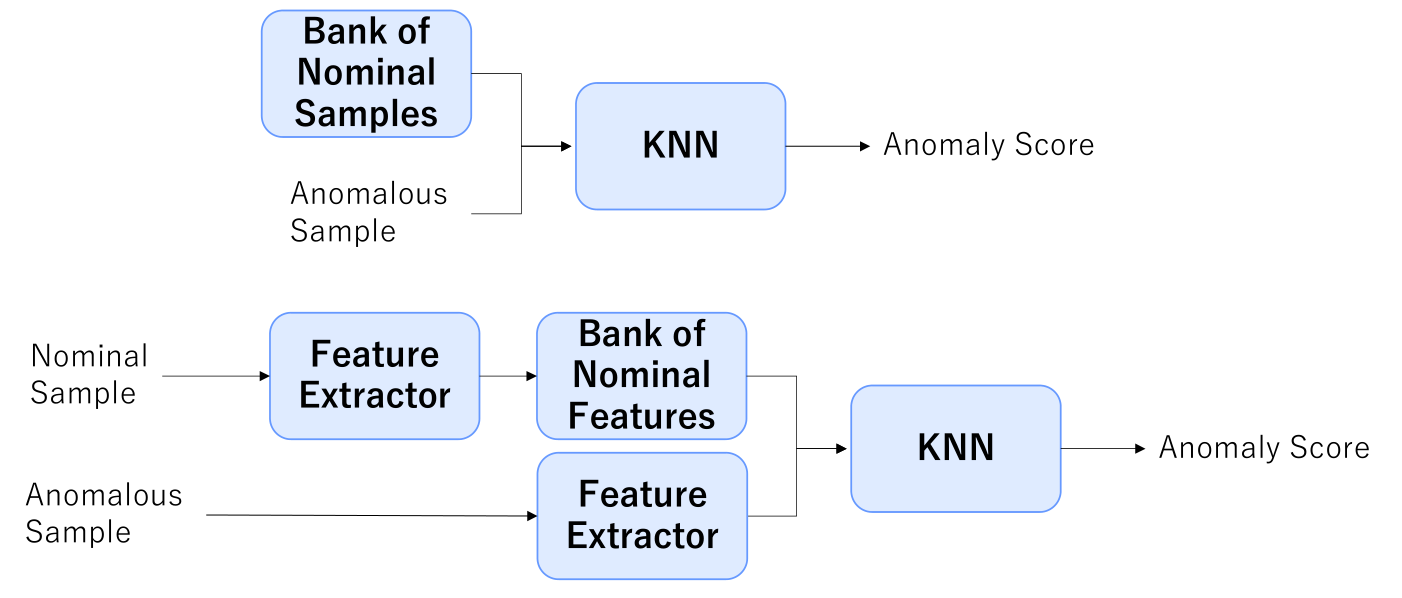
\includegraphics[width=1.0\linewidth]{Chapter_3/feature_extractor_usage.png}
	\end{center}
	\caption{Example of how the pre-trained feature extractor is used in anomaly detection.}
	\label{fig:feature_extractor_usage}
\end{figure} 	

\section{Commonly Used Pre-trained Extractors}
As will be demonstrated by the experiments further in the Chapter~\ref{chapter:ch4} the most commonly used type of models as feature extractors in the industrial anomaly detection models are the convolutional models, specifically residual networks. The case is that residual networks significantly outperform vision transformers as feature extractors for anomaly detection models. This occurrence might be explained by the fact that convolutional models have the higher capacity to capture spatial hierarchies and local relationships than the vision transformer architectures. Throughout all the state-of-the-art industrial anomaly detection models, the common practice is to use feature extractors pre-trained on ImageNet dataset on a supervised classification task. This pre-training on ImageNet allows the models to leverage a vast amount of general knowledge, which can then be fine-tuned to the specific requirements of industrial anomaly detection. ImageNet pre-trained feature extractor are common in all the fields of machine learning including industrial anomaly detection due to the extensiveness and generality of ImageNet dataset. This thesis will further explore these aspects through detailed experiments and analyses, providing a comprehensive understanding of why ResNets remain the backbone of state-of-the-art industrial anomaly detection models.

\subsection{Potential Drawbacks of ImageNet Pre-trained Feature Extractors}
The use of ImageNet pre-trained feature extractors could carry some hidden potential drawbacks when used in industrial anomaly detection. ImageNet dataset consists of wide variety of categories, including manufactured objects alongside with natural samples, humans etc. This diverse nature is indeed beneficial for many general-purpose applications, as it allows for robust feature learning across many domains. Meanwhile, most industrial anomaly detection datasets consist of close up shots of manufactured objects like screws, pills, transistors etc, which require a different focus and precision. As we can observe, the nature of samples found in ImageNet dataset have a discrepancy from the samples that would be found in usual industrial anomaly detection task. Features learned from general purpose datasets such as ImageNet could match industrial features with less accuracy than a feature learned from a specialized dataset. Therefore, it raises the question of whether the apparent convenience of using such well-established models truly outweighs the potential benefits of training models on more specialized datasets tailored to specific industrial needs. We can solidify the assumption by looking at the figure \ref{fig:discrepancy}.

\begin{figure}[h]
	\begin{center}
		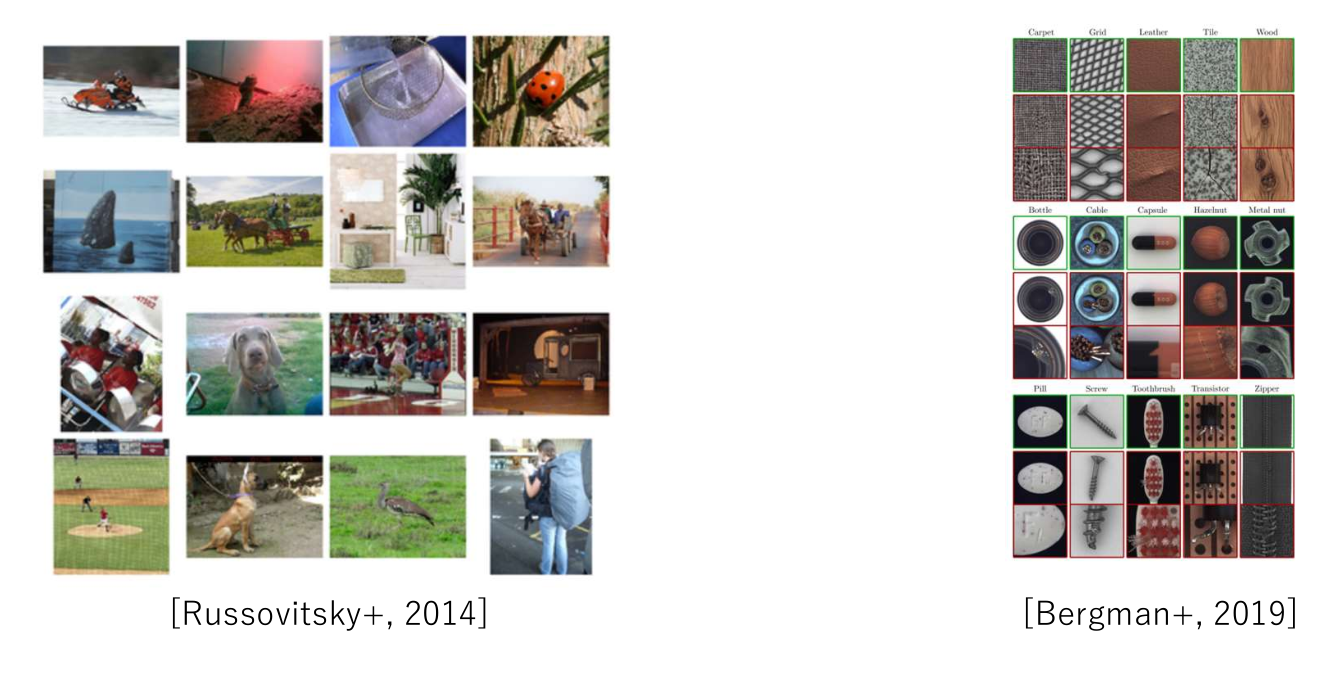
\includegraphics[width=1.0\linewidth]{Chapter_3/discrepancy.png}
	\end{center}
	\caption{Visual comparison of the samples from a common anomaly detection dataset and ImageNet.}
	\label{fig:discrepancy}
\end{figure} 	

\section{Addressing the Drawbacks Through Exploration of Various Feature Spaces}
To test the hypothesis stated above, in this thesis, we decided to test the performance of multiple pre-trained feature extractors on the against each other on the same industrial anomaly detection models. Firstly, we want to find out which architectures would learn the most effective features from the datasets we are going to construct in the future steps. Our goal is not only to identify the most suitable architecture but also to gain insight into how different architectures handle industrial data, especially given the unique challenges presented by these datasets. In order to determine the best architecture we test multiple ImageNet pre-trained models with different architectures on the identical industrial anomaly detection model. Further, after the result of this analysis on model architecture, we move on to the exploration of methods for generation of suitable feature spaces.

\section{Construction of Industrial Anomaly Detection Specialized Feature Spaces}
There are multiple approaches to constructing the possibly suitable feature spaces for industrial tasks. These approaches can be separated mainly into two types: methods that involve enhancing or modifying the feature spaces extracted from ImageNet dataset, methods that consist of assembling a dataset that would be closely related to industrial setting. An example for the first method would be introducing random or synthetic noise to the randomly selected features learned from ImageNet. In this thesis, however, we mainly focus on, and propose multiple ways to accomplish feature space generation by the second method. First approach we explore is the extracting industrial subset from the large scale, general purpose dataset using a CNN classifier as an extractor and learning feature form that subset. Second approach is similar to the first one, with the exception that, instead of using a CNN classifier, we utilize the combination of an LLM and a VLM. (figure \ref{fig:selective_extraction})

\begin{figure}[h]
	\begin{center}
		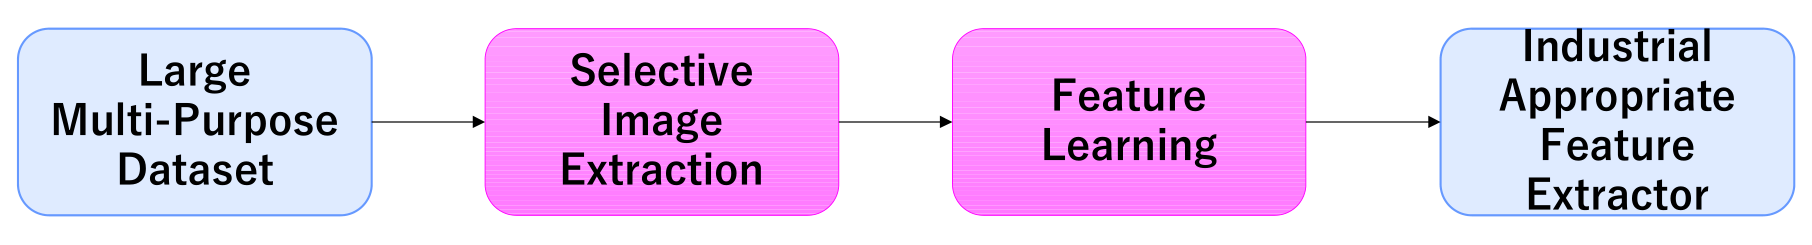
\includegraphics[width=1.0\linewidth]{Chapter_3/selective_extraction.png}
	\end{center}
	\caption{The selective extraction pipeline.}
	\label{fig:selective_extraction}
\end{figure} 	

\section{Selective Extraction With Bi-Class CNN Classifier}
\label{cnn extraction}
As mentioned before, first approach we will be discussing thoroughly is utilizing a bi-class CNN classifier to extract a industrial setting specific subset from the a large scale multi purpose dataset. The process consists of two stages, which are training the bi-class CNN classifier and selecting for industrial images using the trained model. The bi-class classifier will be trained to sort images into two classes: industrial and non-industrial. Once the training phase is complete, the classifier will be utilized to filter through the extensive dataset, flagging and selecting images that fall under the industrial category. Our goal is to achieve precise extraction of industrial setting images, from which, further learning of useful industrial specialized features can be achieved. 

\subsection{Assembling the Bi-Class Classifier}
\label{bi-class assemble}
The procedure of training the bi-class CNN classifier is a standard classification task training on the dataset that consists of samples of two classes, which are "industrial" and "non-industrial"(figure \ref{fig:cnn_train_data}). Firstly, we are required a dataset with such classes, which will be acquired by manually splitting labeled multi-purpose dataset. In the case of this thesis, due to its versatility and large scale, the decision has been made to choose the dataset ImageNet. Further, we split the images in the ImageNet dataset by 1000 classes, having 454 industrial classes and 546 non-industrial classes. Finally, in order to achieve a trained CNN classifier model in a more robust way, we can leverage an ImageNet pre-trained model due to the fact that the new built dataset mostly consist of samples from ImageNet dataset.

\begin{figure}[h]
	\begin{center}
		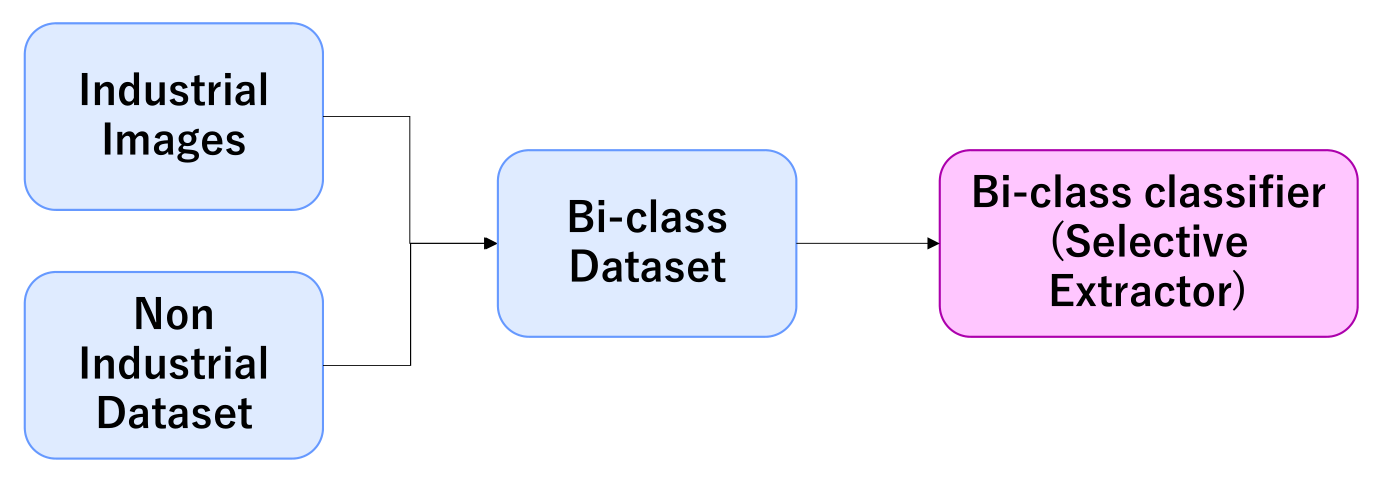
\includegraphics[width=1.0\linewidth]{Chapter_3/cnn_train_data.png}
	\end{center}
	\caption{The construction process of the dataset for the bi-class classifier.}
	\label{fig:cnn_train_data}
\end{figure} 	

The extraction process will be discussed in the next section more thoroughly, however, before moving on to it, an important point should be brought to attention. The point is, after the first selection attempts, through manual visual analysis of the extracted samples, it has been revealed that the extractor model shows bias towards human faces for the "industrial" class. To alleviate this issue, two measures are taken: inclusion of the samples from "Labeled Faces in Wild" into the "non-industrial" subset and extraction of images with prominently shown faces in them using "YOLOv5" object detection. After performing listed actions, the performance of the selective extractor appeared to be acceptable according to manual visual analysis.

\subsection{Selective Extraction}
\label{cnn selective extraction}
Utilizing the CNN selective image extractor, the database for feature learning can be formed(figure \ref{fig:cnn_extraction}). The construction of dataset is performed by classifying images in a large multi-purpose dataset, which is in the case of this work will be the YFCC100M dataset. The choice of this particular dataset is motivated by the necessity of easily accessible and versatile dataset. By performing the classification, the bi-class CNN classifier can effectively sift through the vast YFCC100M dataset, isolating and extracting a subset of images that are assumed to be related to industrial settings. Furthermore, upon visual inspection of the extracted samples, it becomes evident that there is a noticeable bias towards industrial images, indicating the efficacy of the bi-class CNN classifier in accurately identifying and selecting industrial-relevant samples.

\begin{figure}[h!]
	\begin{center}
		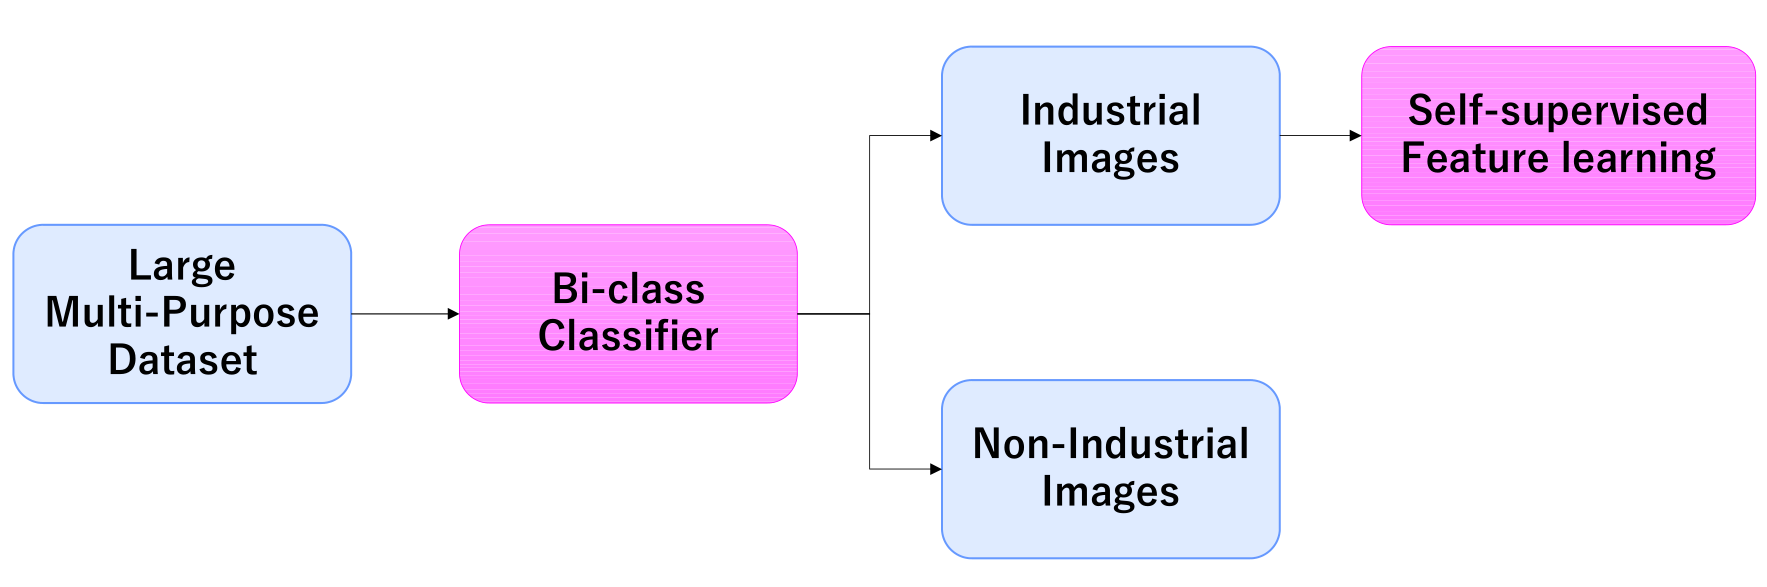
\includegraphics[width=1.0\linewidth]{Chapter_3/cnn_extraction.png}
	\end{center}
	\caption{The process of selective extraction using bi-class classifier.}
	\label{fig:cnn_extraction}
\end{figure} 	

\subsection{Feature Learning}
\label{feature learning cnn}
Due to the nature of the selective extraction method, the resultant dataset comprises solely of the "industrial" class for all the samples extracted. Given that supervised classification task training necessitates the presence of multiple classes within a dataset, utilizing this single-class dataset for such tasks is evidently not feasible. To circumvent this limitation, we opt for an unsupervised learning approach. Specifically, we employ a self-supervised learning model known as DINO to extract meaningful features from the vast, unlabeled dataset of industrial images. For a more in-depth discussion of the DINO model and its underlying mechanisms, readers are referred to Chapter~\ref{chapter:ch2}, where detailed explanations and examples are provided.

\section{Selective Extraction With an LLM and a VLM}
\label{sec:llm_and_vlm_extraction}
The second approach to the selective extraction that is proposed in this thesis is the utilization of the combination of an LLM(Large Language Model) and an VLM(Vision Language Model). The pipeline of the selective extraction by this method consists of two major stages, which are generation of descriptions using an LLM and filtration by a cosine similarity threshold with the help of an VLM. For this work we chose GPT-3 model as the LLM and CLIP model as the VLM. This method can function in specialized manner and in a general manner. When used in a specialized manner, it is possible to generate descriptions that would select for images that are close in feature to a specific use case. In generalized style of functioning, we generate descriptions that are related to the word "industrial", "manufacturing" etc. In the case of this thesis, we focus on improving the performance on the dataset MVTechAD in order to test the efficiency of the method in constrained boundaries. The steps to utilize the method with focus on MVTechAD are as follows: using specific prompts to generate descriptions and extracting images using the CLIP model. Please refer to figure \ref{fig:llm_extraction} for visual explanation of the pipeline.

The first prompt to the GPT-3 model is as follows:

"give a python array containing the word "transistor" and it's synonyms, include as much synonyms as possible but avoid unrelated words"

afterwards, the following prompt is given:

"generate description for use in a CLIP model using these generated words, each word should be used in at least one description. One description should contain at least one word from the list. Generate as much descriptions as possible. Output as python array"

This process generates description for a single category in the MVTechAD dataset. Further, the same procedure is applied to the remaining categories in the dataset. We also generate descriptions using the templates: "This is x" and "This is a photo of x".

To determine the threshold value that is used for the extraction process, we apply CLIP with the descriptions specific to a category in the MVTechAD dataset to the images in the same category. Through the aforementioned approach the value of 0.29 was determined to be optimal to extract images. Every image that passes the threshold 0.29 on any of the descriptions are selected from the YFCC100M dataset. 

\begin{figure}[h]
	\begin{center}
		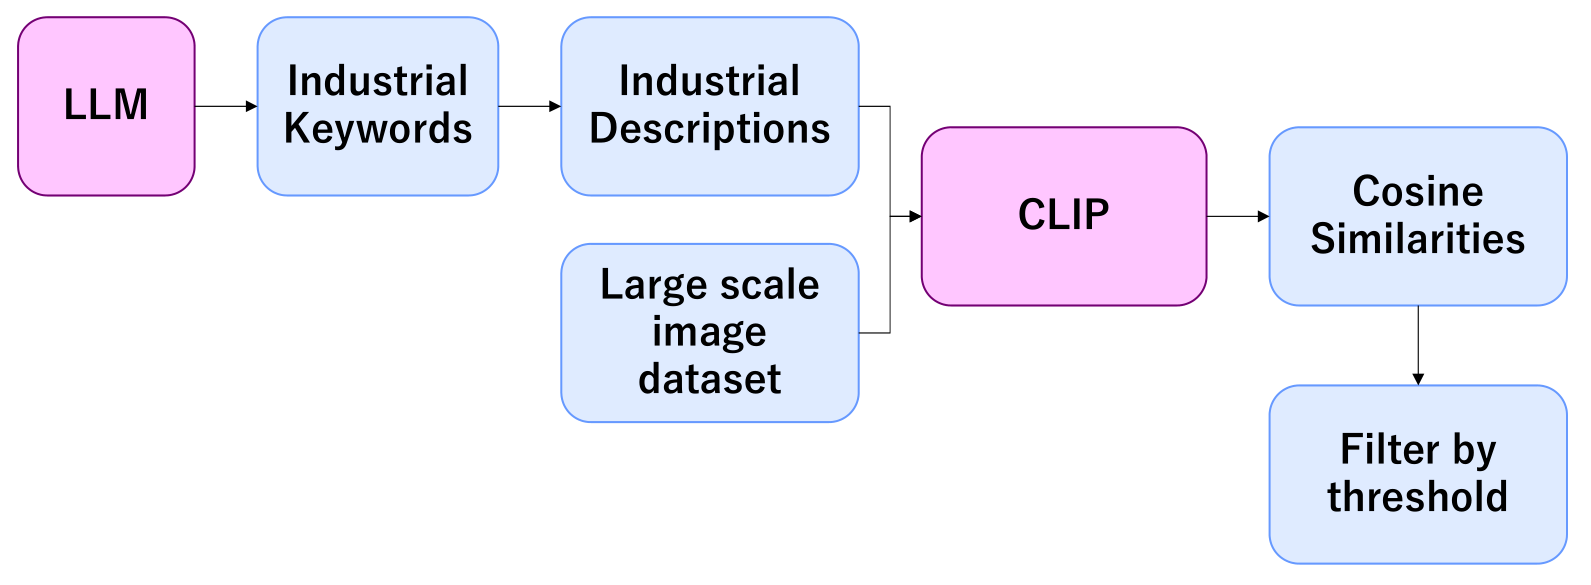
\includegraphics[width=1.0\linewidth]{Chapter_3/llm_extraction.png}
	\end{center}
	\caption{The pipeline of selective extraction using an LLM and a VLM.}
	\label{fig:llm_extraction}
\end{figure} 	

\subsection{Feature Learning}
\label{feature learning llm}
The use of base keywords, which are in this case categories from MVTechAD dataset, makes it possible to assemble a labeled dataset, unlike the method with the bi-class CNN classifier. This property of the method of extraction creates a possibility of feature learning through supervised classification task training. Supervised learning is accomplished by using the base keywords that are given in the former prompts, which are, in the of this thesis, the categories in the dataset MVTechAD. Moreover, we use the features of the ImageNet pre-trained model as the starting point and perform a fine-tuning instead of learning features from scratch. The performance of ImageNet features on the industrial anomaly detection makes them a good starting point for training.

%insert feature learning graphic
%%
%%% Chapter 4
\cleardoublepage
\chapter{Experiments, Results and Implementation}
\label{chapter:ch4}

In this chapter the process and results of multiple experiments, that look into performance of various pre-trained feature extractors in industrial anomaly detection tasks, will be presented. First experiment serves to determine the layers of vision transformer architecture that would provide the highest accuracy for anomaly detection when applied as backbones. Secondly, the analysis on the efficacy of self-supervised model DINO against supervised classification task training, helping us to make the decision for verifying the method for feature learning. Next, we will provide a performance comparison between different types of deep learning visual models as feature extractors on the PatchCore model, in order to determine which architecture should be chosen for further experiments. Further, we test the feature space learned from the dataset constructed by the method of selective extraction using CNN bi-class classifiers. Generated feature space competes against one of the state-of-the-art feature spaces for industrial anomaly detection: WideResNet50. Lastly, we will engage in a comparative analysis of the efficiency of the feature space based on a dataset extracted through a method that employs both large language models (LLMs) and visual language models (VLMs). Through these comprehensive experiments and analyses, we aim to derive valuable insights and optimal approaches for advancing industrial anomaly detection by approaching the task as a feature space problem.

\section{Scoring methodology}

\subsection{Scoring metric}
For all the experiments, in order to measure the accuracy of the models being tested, we use AUROC (Area Under the Receiver Operating Characteristic curve) metric. AUROC metric represent the models capability to determine true positives while keeping the number of false positives relatively low. ROC curve, as shown in the figure \ref{fig:auroc}, is the curve that represents the relationship between TPR and FPR at any given threshold. TPR and FPR at an arbitrary threshold is calculated by equations \ref{eq:tpr} and \ref{eq:fpr} respectively. AUROC score is represented as a number between 0 and 1.0(higher the better) and generally, the score 0.5 represents the random guessing. Therefore, scores below 0.5 are considered worse than random guessing while above 0.5 are better. Figures in this paper represent the AUROC score as the percentage from 0\% to 100\%.

\begin{equation}
	TPR = \frac{\text{True Positives}}{\text{True Positives} + \text{False Negatives}}
	\label{eq:tpr}
\end{equation}

\begin{equation}
	FPR = \frac{\text{False Positives}}{\text{False Positives} + \text{True Negatives}}
	\label{eq:fpr}
\end{equation}

\begin{figure}[h]
	\begin{center}
		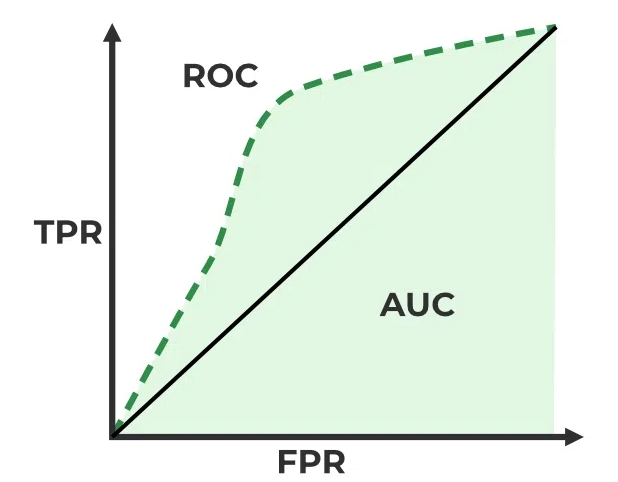
\includegraphics[width=0.5\linewidth]{Chapter_4/auroc.png}
	\end{center}
	\caption{Medical Visual Question Answering (VQA) \cite{liu2021slake} is a task where the model receives medical images and corresponding questions as input and produces accurate answers as the output.}
	\label{fig:auroc}
\end{figure}

\subsection{Industrial Anomaly detection model}
The model of choice for all the tests is the PatchCore model, as it allows an easy plug and play approach to pre-trained feature extractors. PatchCore outputs three types of scores for each category in the MVTechAd dataset. There are also mean scores over all cotegories provide for each type of scores. Types of scores are as follows:

\begin{description}
  \item[Instance AUROC] represents AUROC score for classifying each image as anomalous or nominal
  \item[Anomaly Pixel AUROC] represents AUROC score for classifying each pixel as anomalous or nominal, calculated only on images that contain anomalies
  \item[Full Pixel AUROC] represents AUROC score for classifying each pixel as anomalous or nominal, calculated over all images
\end{description}

In order to be able to utilize Vision Transformer architectures with PatchCore model, the following changes have been made. These changes detect if the ViT is being used as pre-trained feature extractor and reshape the layers as appropriate for PatchCore.

\lstset{frame=tb,
  language=Python,
  aboveskip=3mm,
  belowskip=3mm,
  showstringspaces=false,
  columns=flexible,
  basicstyle={\small\ttfamily},
  numbers=none,
  numberstyle=\tiny\color{gray},
  breaklines=true,
  breakatwhitespace=true,
  tabsize=3
}
\begin{lstlisting}
def patchify(self, features, return_spatial_info=False):
	#...
	if len(features.shape) == 3:
		features = features.transpose(1, 2)
		if features.shape[2] == 197:
			features = features[:, :, 1:]
		hw = int(math.sqrt(features.shape[2]))
		features = features.view(features.shape[0], features.shape[1], hw, hw)
	#...
\end{lstlisting}

\section{Comparison of ViT layers}
\label{vit layers}

In the first experiment we will be analysing the difference of the layers of vision transformer architectures. Throughout the experiment we use VitB/16 pre-trained on ImageNet classification task. PatchCore research paper recommend using the features from one layer, or aggregating features from up to two layers in order to achieve best results. The results in the figure \ref{fig:vit_layers} indicate Instance AUROC mean scores across all the categories in the dataset MVTechAd. As displayed in the figure \ref{fig:vit_layers}, the best approach is the utilization of the layer 8 alone. This approach achieves the highest score of 94.38\%. For all the experiments involving Vision Transformer architecture, we will be opting for layer 8 of VitB/16 model.

\begin{figure}[h]
	\begin{center}
		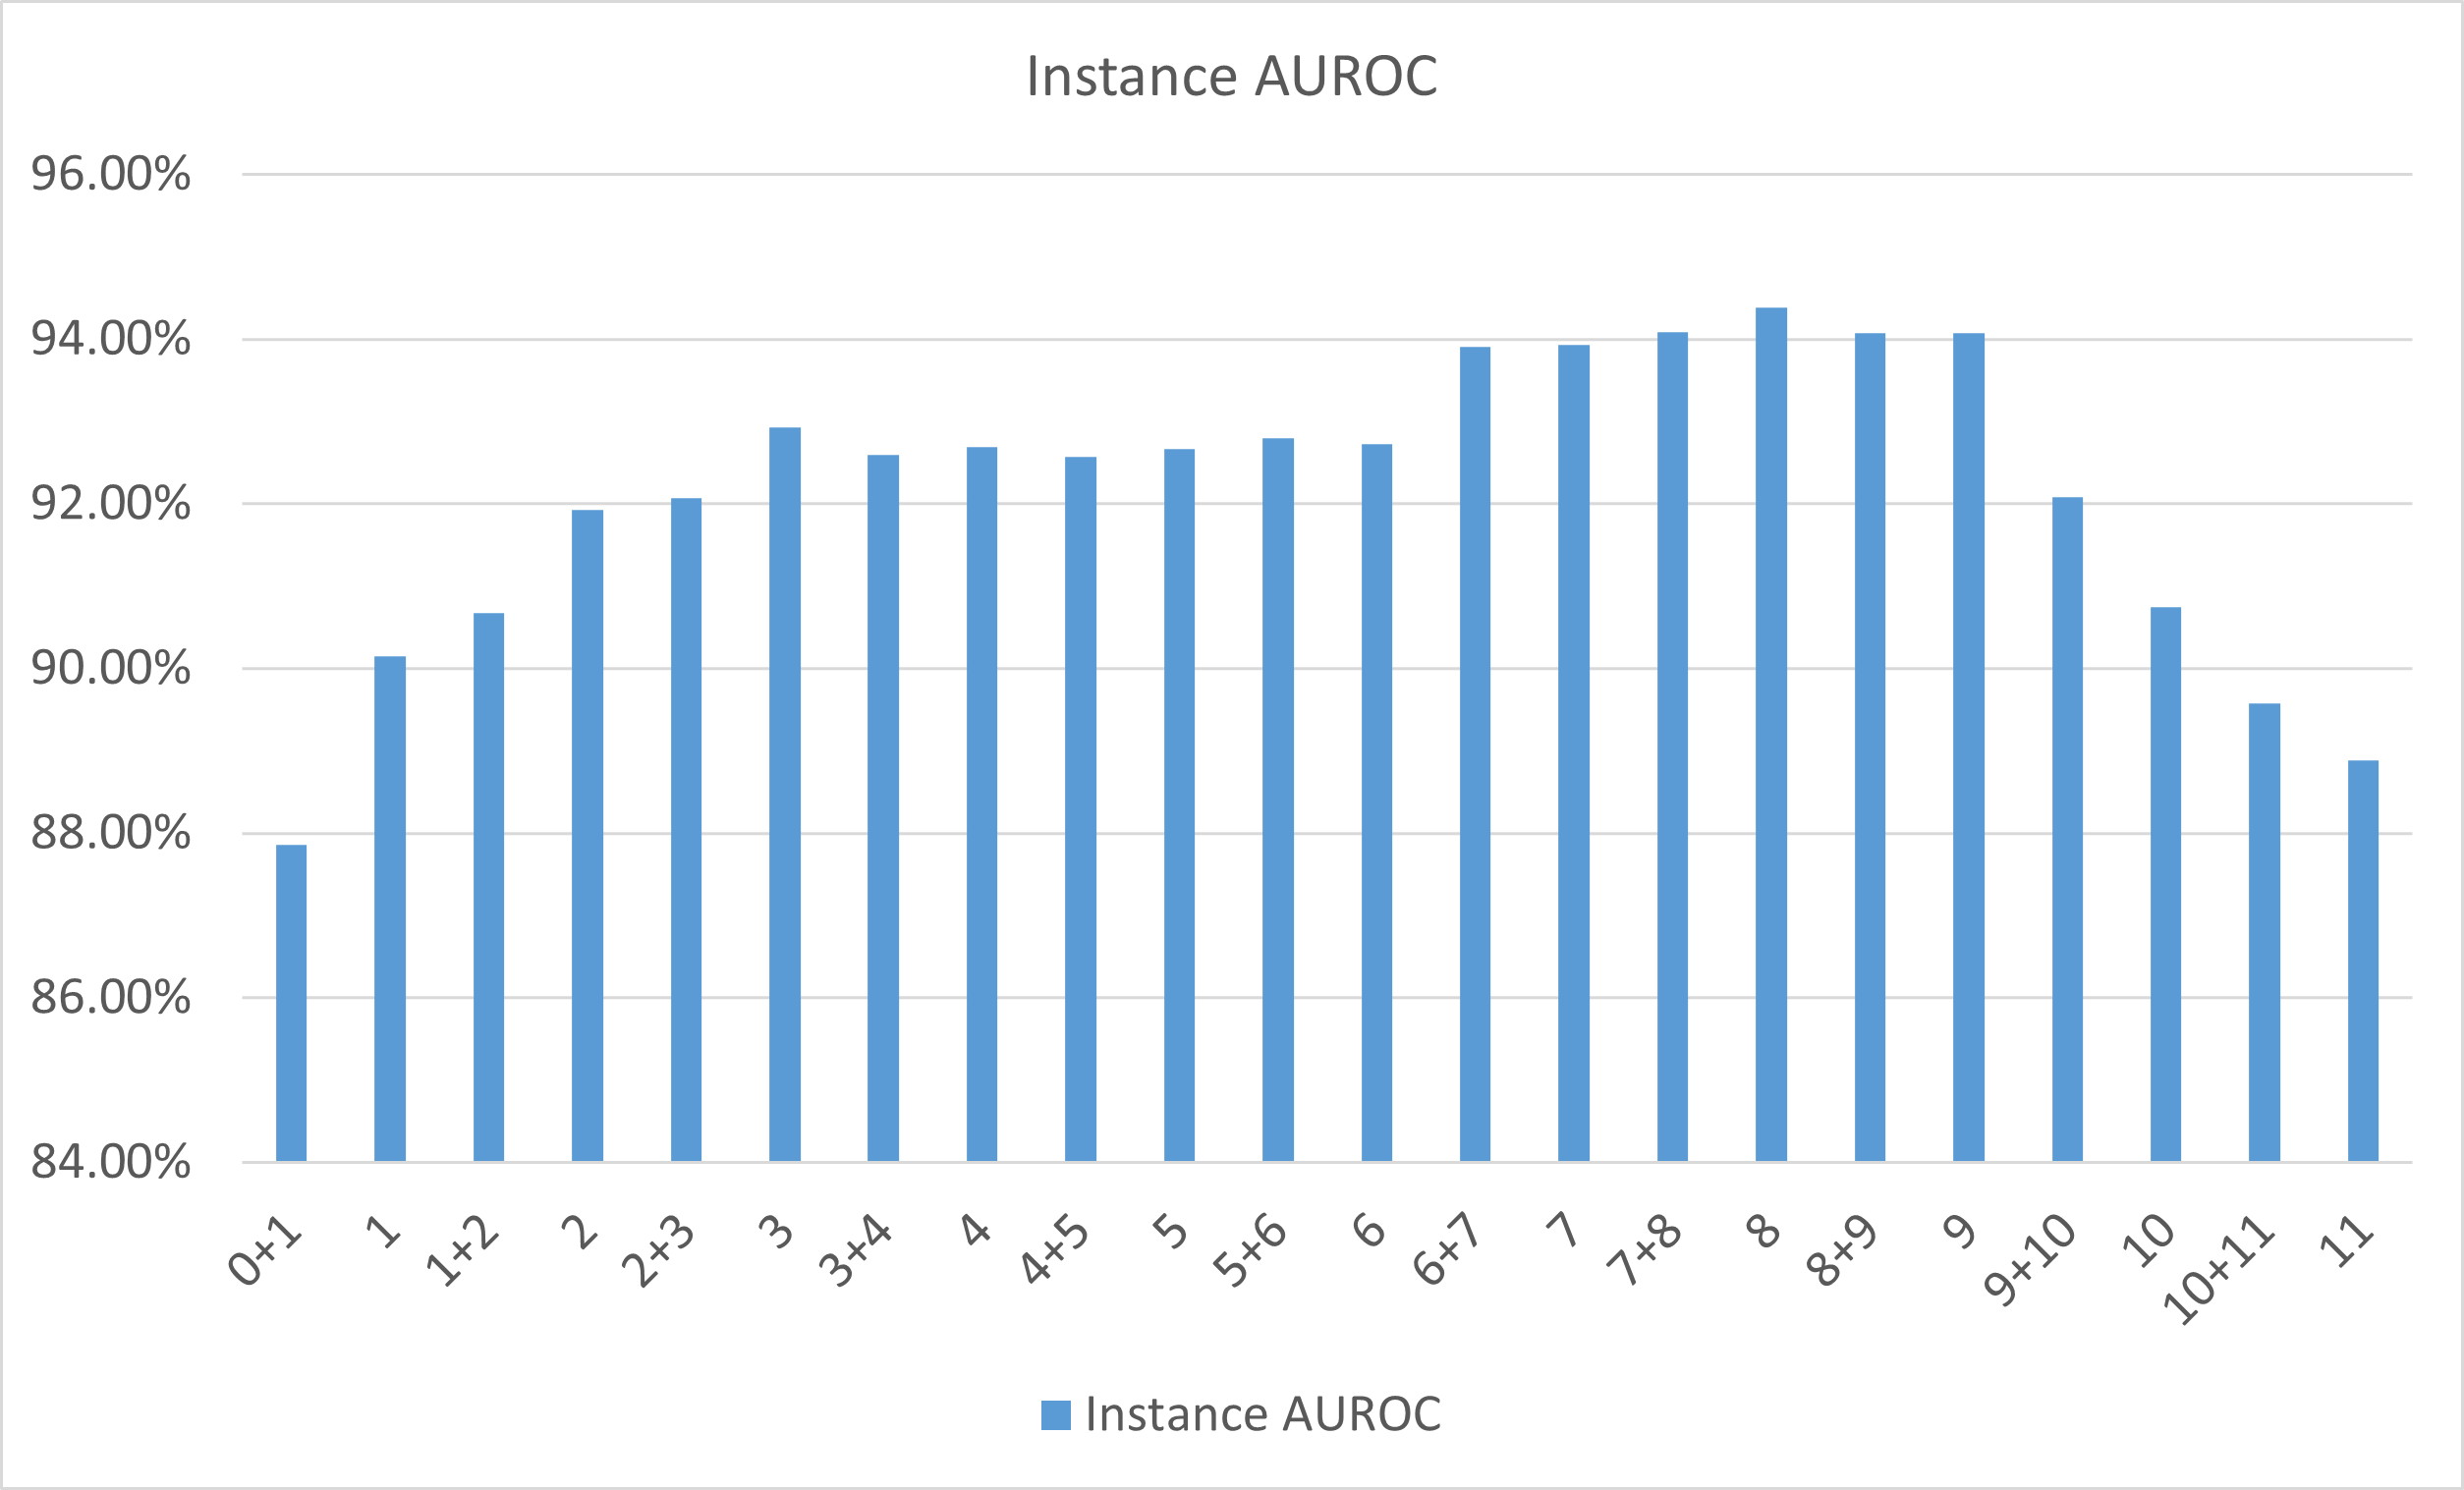
\includegraphics[width=1.0\linewidth]{Chapter_4/vit.png}
	\end{center}
	\caption{Mean Instance AUROC score across all categories of MVTechAd for PatchCore with VitB/16 pre-trained extractor}
	\label{fig:vit_layers}
\end{figure}

\section{Superiority of WideResNet50 over ResNet50}
In the following experiment we show that WideResNet50 architecture has an overhead of efficiency against ResNet50 architecture. Analysing the figure \ref{fig:resnet_vs_wideresnet} we can clearly see that WideResNet50 has better performances in all the mean scores. Following this discovery, and the conclusion from the next experiment, we opt for the usage of WideResNet50 model to learn features from extracted datasets.

\begin{figure}[h]
	\begin{center}
		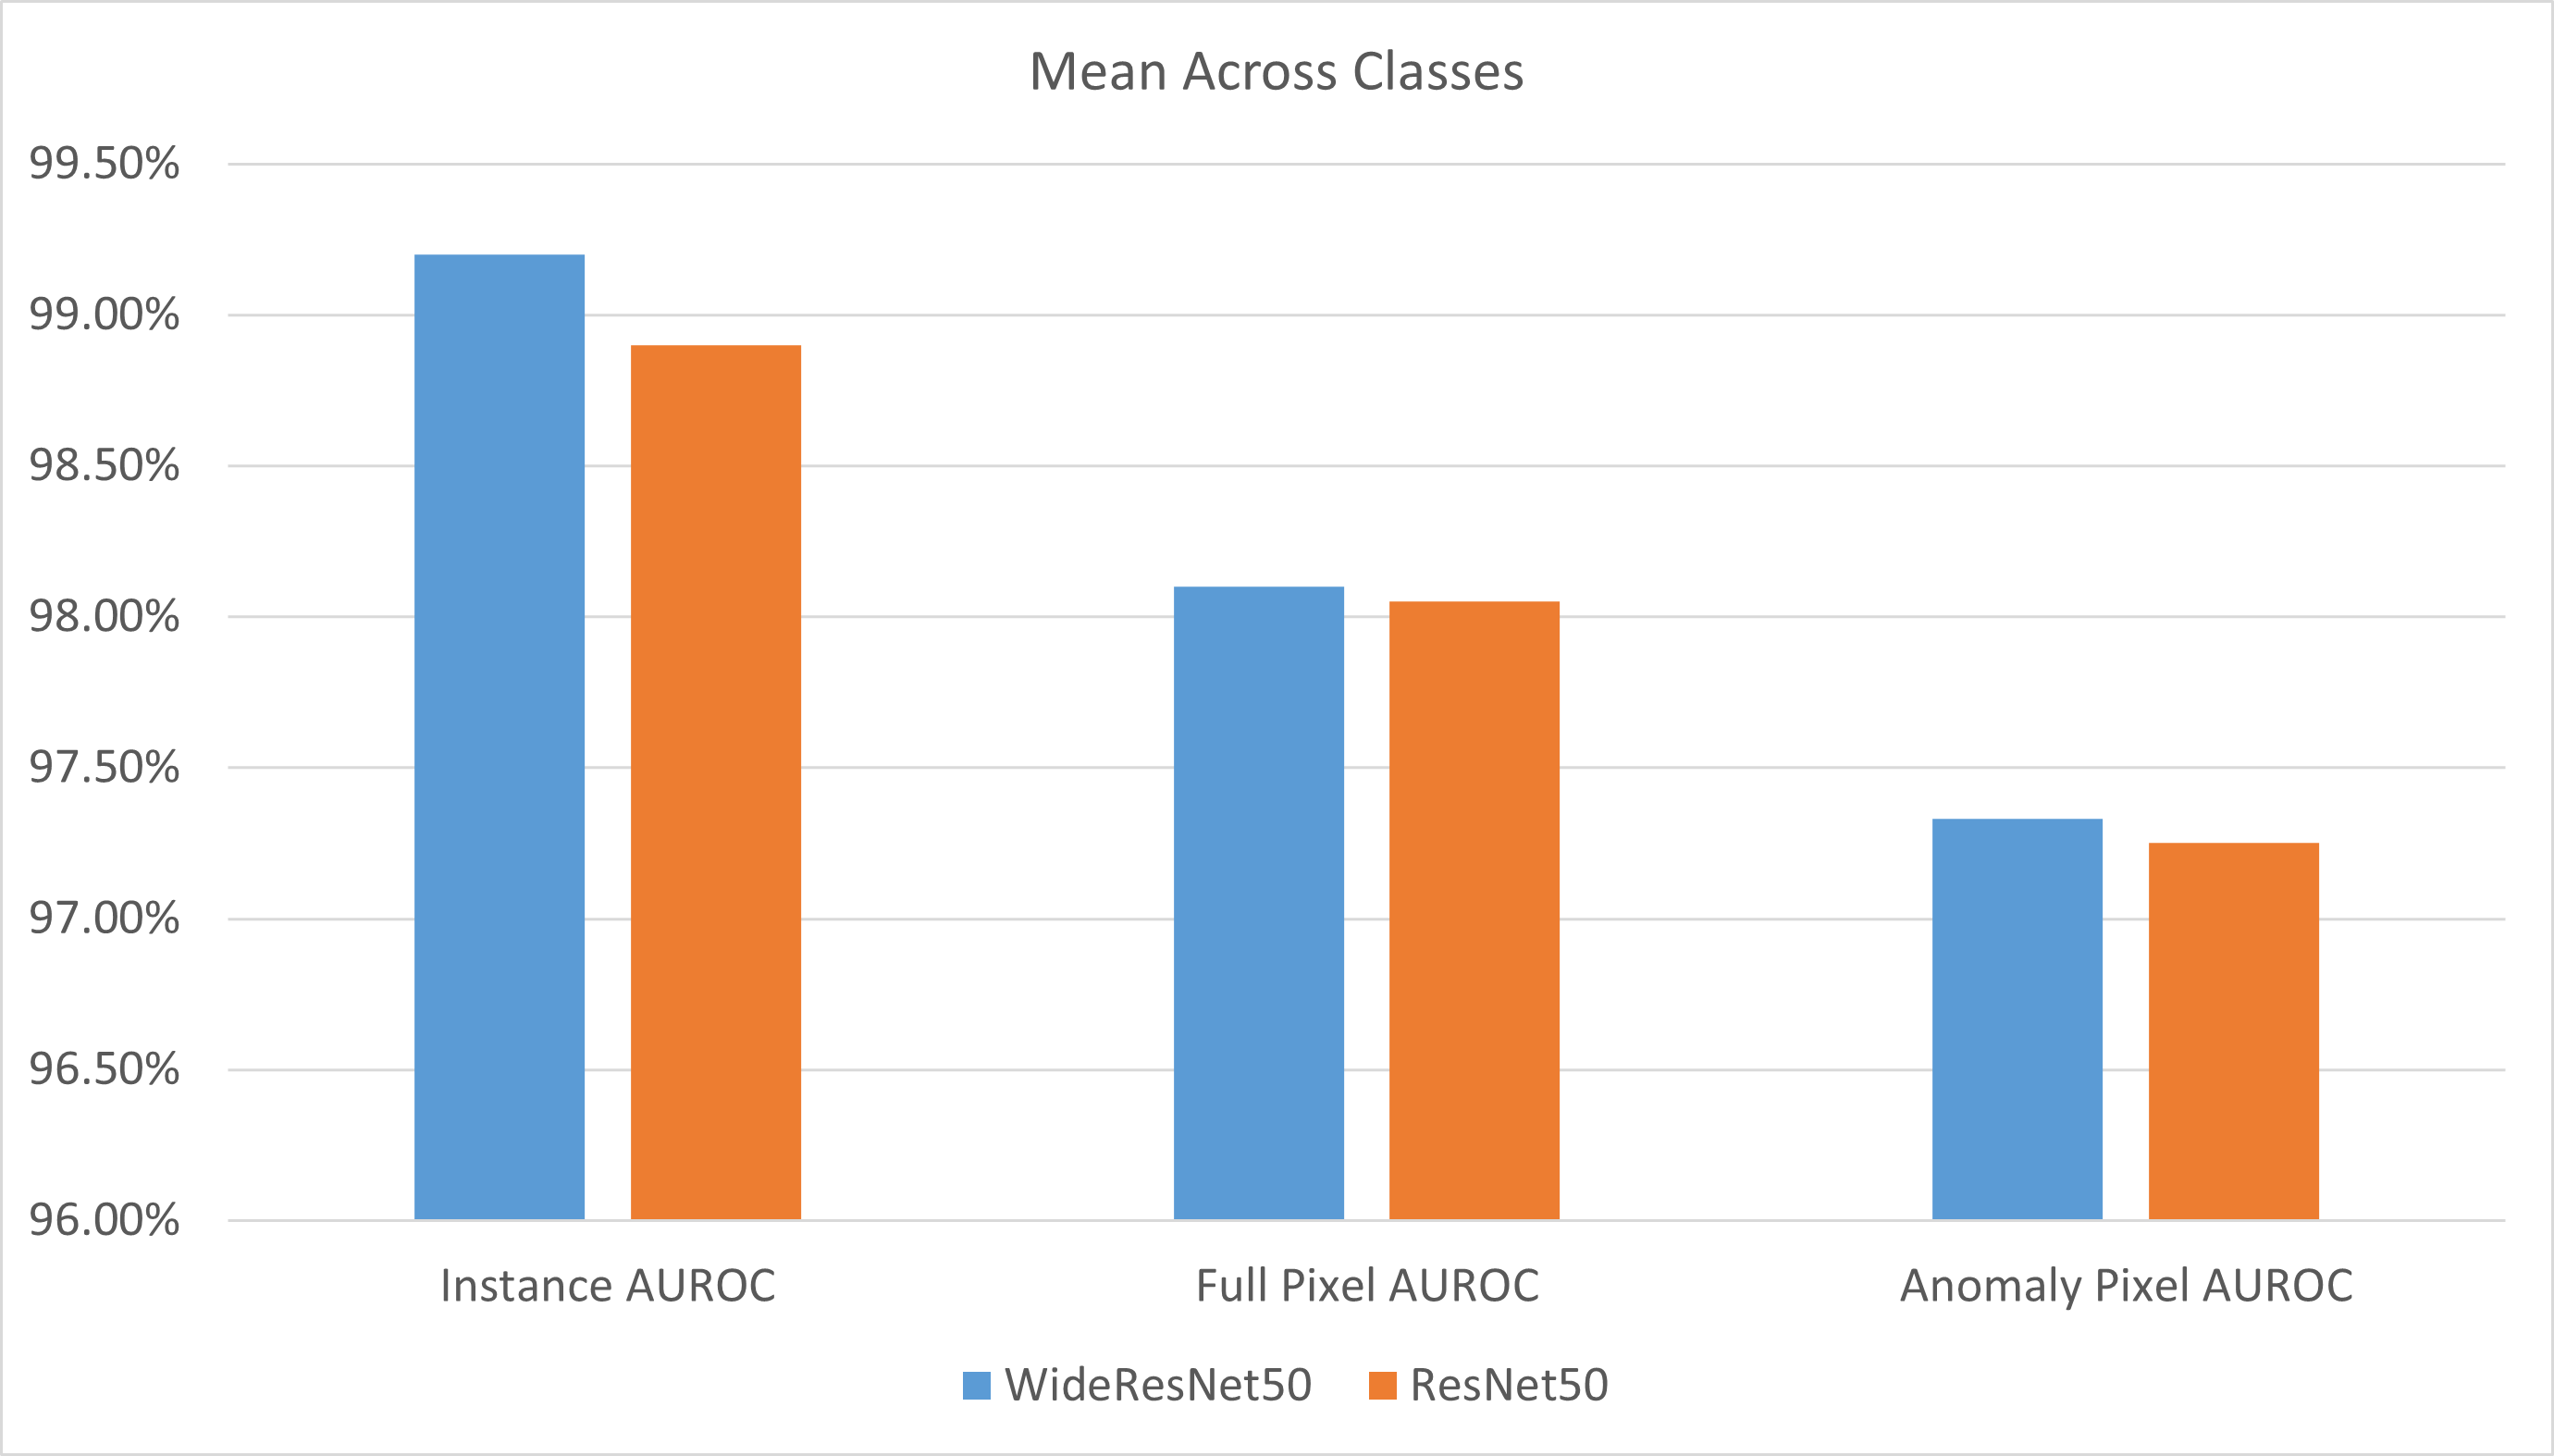
\includegraphics[width=1.0\linewidth]{Chapter_4/resnet_vs_wideresnet.png}
	\end{center}
	\caption{Mean Instance AUROC score across all categories of MVTechAd for PatchCore with VitB/16 pre-trained extractor}
	\label{fig:resnet_vs_wideresnet}
\end{figure}

\section{Analysis on the efficieny of DINO model}
\label{sec:dino_tests}
In this experiment we aim to determine if the self-supervised training model is capable enough to compete with the supervised learning methods in generating feature spaces for the use in IAD models. We compare ResNet50 model the pre-trained using supervised classification method by the PyTorch team and ResNet50 pre-trained using DINO self-supervised learning mode. Both models are trained on ImageNet1K dataset. Below we provide recipes for training each model.

PyTorch pre-trained ResNet50:

\lstset{frame=tb,
  language=bash,
  aboveskip=3mm,
  belowskip=3mm,
  showstringspaces=false,
  columns=flexible,
  basicstyle={\small\ttfamily},
  numbers=none,
  numberstyle=\tiny\color{gray},
  breaklines=true,
  breakatwhitespace=true,
  tabsize=3
}
\begin{lstlisting}
torchrun --nproc_per_node=8 train.py --model $MODEL_NAME --batch-size 128 \ 
--lr 0.5 --lr-scheduler cosineannealinglr --lr-warmup-epochs 5 \
--lr-warmup-method linear --auto-augment ta_wide --epochs 600 \ 
--random-erase 0.1 --weight-decay 0.00002 --norm-weight-decay 0.0 \ 
--label-smoothing 0.1 --mixup-alpha 0.2 --cutmix-alpha 1.0 \
--train-crop-size 176 --model-ema --val-resize-size 232
\end{lstlisting}

DINO pre-trained ResNet50:

\lstset{frame=tb,
  language=json,
  aboveskip=3mm,
  belowskip=3mm,
  showstringspaces=false,
  columns=flexible,
  basicstyle={\small\ttfamily},
  numbers=none,
  numberstyle=\tiny\color{gray},
  breaklines=true,
  breakatwhitespace=true,
  tabsize=3
}
\begin{lstlisting}
{
	"arch": "resnet50", 
	"out_dim": 60000, 
	"norm_last_layer": true, 
	"warmup_teacher_temp": 0.04, 
	"teacher_temp": 0.07, 
	"warmup_teacher_temp_epochs": 50, 
	"use_fp16": false, 
	"weight_decay": 0.000001, 
	"weight_decay_end": 0.000001, 
	"clip_grad": 0, 
	"batch_size_per_gpu": 51, 
	"epochs": 800, 
	"freeze_last_layer": 1, 
	"lr": 0.3, 
	"warmup_epochs": 10, 
	"min_lr": 0.0048, 
	"global_crops_scale": [0.14, 1.0], 
	"local_crops_scale": [0.05, 0.14], 
	"local_crops_number": 6, 
	"seed": 0, 
	"num_workers": 10, 
	"world_size": 80, 
	"optimizer": "lars", 
	"momentum_teacher": 0.996, 
	"use_bn_in_head": true
}
\end{lstlisting}

The figure \ref{fig:dino_test} shows the mean scores Instance AUROC, Full Pixel AUROC and Anomaly Pixel AUROC across all categories of MVTechAd dataset. From the data presented in the figure we can conclude that DINO self-supervised method can outperform supervised classification learning when trained with a correct recipe. As it is shown, in this case, DINO model outperforms supervised method by 0.07\% in Instance AUROC, 0.15\% in Full Pixel AUROC and 0.27\% in Anomaly Pixel AUROC. Based on these findings we can move forward using the DINO self-supervised learning model for our feature learning purposes.

\begin{figure}[h]
	\begin{center}
		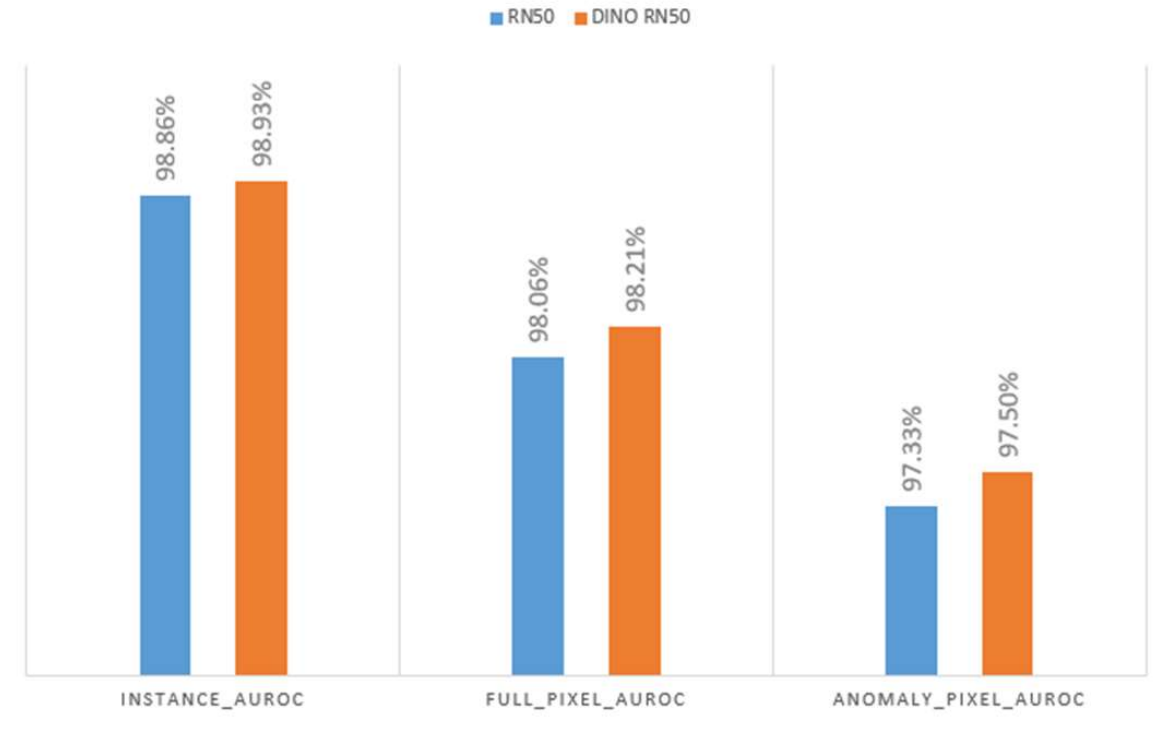
\includegraphics[width=1.0\linewidth]{Chapter_4/dino.png}
	\end{center}
	\caption{Mean scores Instance AUROC, Full Pixel AUROC and Anomaly Pixel AUROC across all categories of MVTechAd dataset}
	\label{fig:dino_test}
\end{figure}

\section{CNN bi-class classifier selective extraction experiments}
\label{sec:comp_vis}

\subsection{Training the CNN bi-class classifier}
We are going to put together a dataset in order to train a CNN bi-class classifier with the method indicated in the Chapter~\ref{chapter:ch3}. The datasets is assembled with the method displayed in the figure \ref{fig:bi_class_prep}. Industrial class of the dataset contains: 454 classes from ImageNet with the removal of images that contain faces prominently, also it contains multiple industrial datasets that are stated in the figure \ref{fig:bi_class_prep}. It is important to note that, the industrial datasets included in the industrial class of the dataset for the training of CNN bi-class classifier, do not reflect on the final learned features that are used in the PatchCore model during test time. We assemble the non-industrial part of the dataset by using 546 classes from ImageNet dataset and Labeled Faces in Wild dataset.

\begin{figure}[h]
	\begin{center}
		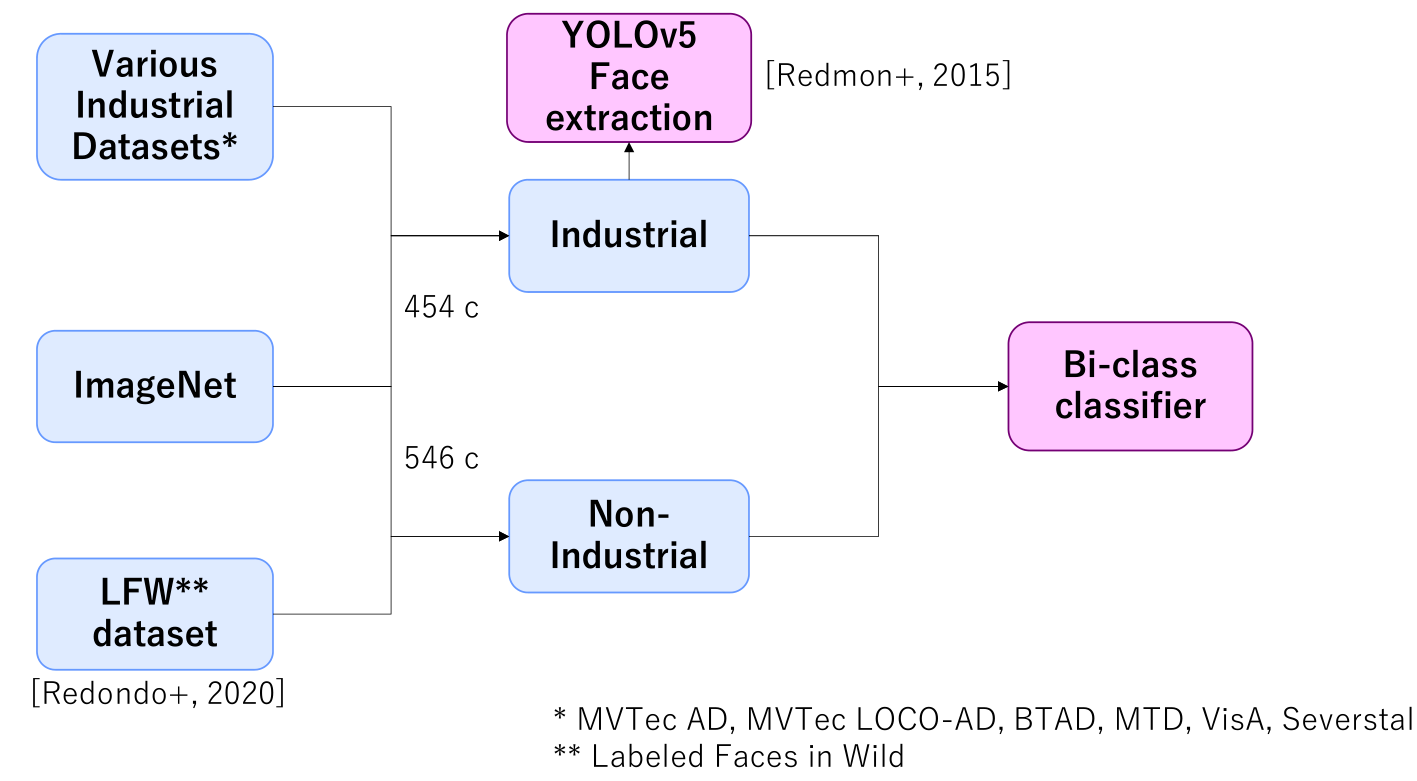
\includegraphics[width=1.0\linewidth]{Chapter_4/bi_class_prep.png}
	\end{center}
	\caption{Mean scores Instance AUROC, Full Pixel AUROC and Anomaly Pixel AUROC across all categories of MVTechAd dataset}
	\label{fig:bi_class_prep}
\end{figure}

Using the constructed dataset the extractor model is trained by fine-tuning ImageNet pre-trained ResNet50 model for 25 epochs. The recipe for the fine-tuning is as follows:

\lstset{frame=tb,
  language=Python,
  aboveskip=3mm,
  belowskip=3mm,
  showstringspaces=false,
  columns=flexible,
  basicstyle={\small\ttfamily},
  numbers=none,
  numberstyle=\tiny\color{gray},
  breaklines=true,
  breakatwhitespace=true,
  tabsize=3
}
\begin{lstlisting}
def fine_tune():
	model_ft = models.resnet50(weights='IMAGENET1K_V1')
	num_ftrs = model_ft.fc.in_features
	model_ft.fc = nn.Linear(num_ftrs, len(class_names))
	model_ft = model_ft.to(device)
	criterion = nn.CrossEntropyLoss()
	optimizer_ft = optim.Adam(model_ft.parameters(), lr=0.001)
	exp_lr_scheduler = lr_scheduler.StepLR(optimizer_ft, step_size=7, gamma=0.1)
	model_ft = train_model(model_ft, criterion, optimizer_ft, exp_lr_scheduler, num_epochs=20)
	torch.save(model_ft.state_dict(), 'fine_tuned.pt')
\end{lstlisting}

\subsection{Selective extraction of the dataset for feature learning}
We utilize the trained CNN bi-class classifier to extract an industrial specialized dataset from the YFCC100M dataset. We use the following method to extract the desired samples from the large dataset:


\lstset{frame=tb,
  language=Python,
  aboveskip=3mm,
  belowskip=3mm,
  showstringspaces=false,
  columns=flexible,
  basicstyle={\small\ttfamily},
  numbers=none,
  numberstyle=\tiny\color{gray},
  breaklines=true,
  breakatwhitespace=true,
  tabsize=3
}
\begin{lstlisting}
def predict_image(image_name):
    image = image_loader(image_name)
    with torch.no_grad():
        logits = model.forward(image)
    ps = torch.exp(logits)
    _, predTest = torch.max(ps, 1)
    return predTest[0]

cnt = 0

for (root, dirs, files) in os.walk(address, topdown=True):
    cnt = cnt + 1
    for f in files:
        if f.endswith(".jpg"):
            try:
                t = predict_image(os.path.join(root, f))
            except:
                print(os.path.join(root, f))
            if t == 0:
                os.makedirs(os.path.join(addressDest, str(cnt//1000)), exist_ok=True)
                shutil.copy2(os.path.join(root, f), os.path.join(addressDest, str(cnt//1000), f))
\end{lstlisting}

Here, model refers to bi-class CNN classifier model. After applying this proces to the YFCC100M dataset for a limited amount of time, we receive 2 343 499 industrial samples.

\subsection{Learning features using DINO VitB/16 model}
First batch of feature space comparisons include the state-of-the-art feature extractor ImageNet pre-trained WideResNet50, ImageNet pre-trained VitB/16 and VitB/16 trained with self-supervised learning method DINO. The recipe for training the ImageNet pre-trained WideResNet50 and ImageNet pre-trained VitB/16 is the same as the recipe for ResNet50 stated in the section \ref{sec:dino_tests}. The recipe for the training of VitB/16 on the extracted dataset is as follows (Here, "/po1/rakhimov/extracted" is the extracted dataset.):

\lstset{frame=tb,
  language=bash,
  aboveskip=3mm,
  belowskip=3mm,
  showstringspaces=false,
  columns=flexible,
  basicstyle={\small\ttfamily},
  numbers=none,
  numberstyle=\tiny\color{gray},
  breaklines=true,
  breakatwhitespace=true,
  tabsize=3
}
\begin{lstlisting}
torchrun --nnodes=1 --nproc_per_node=4 main_dino.py --arch vit_base \
--data_path /po1/rakhimov/extracted --output_dir /po1/rakhimov/result \ 
--epochs 100
\end{lstlisting}

It can be understood from the data displayed in the figure \ref{fig:vit_custom_test} that Vision Transformer architecture performs noticably less than CNN architecture. We can draw said conclusion by analysing the performances of ImageNet pre-trained WideResNet50 and VitB/16. Differences in performance are: 6.22\% for Instance AUROC, 2.47\% for Full Pixel AUROC and 2.8\% for Anomaly Pixel AUROC. When it comes to the extracted dataset, although we have efficiency improvement upon VitB/16 trained on ImageNet, overall performance gain over the state-of-the-art feature extractor has not been achieved. Moreover, from this experiment we can conclude that Vision Transformer architecture is unadvisible to use in the further experiments.

\begin{figure}[h]
	\begin{center}
		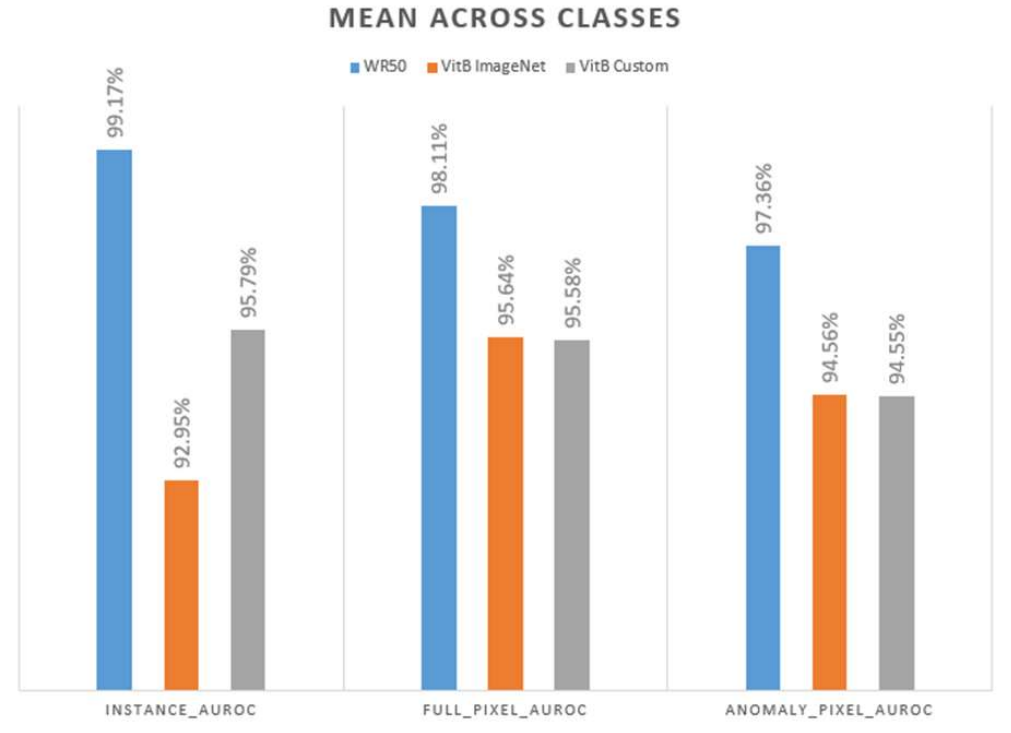
\includegraphics[width=1.0\linewidth]{Chapter_4/vit_custom.png}
	\end{center}
	\caption{Mean scores Instance AUROC, Full Pixel AUROC and Anomaly Pixel AUROC across all categories of MVTechAd dataset}
	\label{fig:vit_custom_test}
\end{figure}

\subsection{Learning features using DINO self-supervised method with the WideResNet50 model}
After the conclusions from the last experiments, we train WideResNet50 using DINO self-supervised method on the extracted dataset. In order to test the efficacy of the selection method, we also train WideResNet50 using the same recipe on 2 343 499 randomly extracted from the YFCC100M dataset. The recipe to train WideResNet50 is as follows:

\lstset{frame=tb,
  language=bash,
  aboveskip=3mm,
  belowskip=3mm,
  showstringspaces=false,
  columns=flexible,
  basicstyle={\small\ttfamily},
  numbers=none,
  numberstyle=\tiny\color{gray},
  breaklines=true,
  breakatwhitespace=true,
  tabsize=3
}
\begin{lstlisting}
torchrun --nproc_per_node=8 main_dino.py --arch wide_resnet50_2 \ 
--optimizer sgd --lr 0.03 --weight_decay 1e-4 \ 
--weight_decay_end 1e-4 --global_crops_scale 0.14 1 \ 
--local_crops_scale 0.05 0.14 --data_path /po1/rakhimov/extracted \ 
--output_dir /po1/rakhimov/result_wd50 --epochs 100
\end{lstlisting}

We also include ResNet50 pre-trained on ImageNet using DINO self-supervised learning method, in order to compare the ImageNet to the extracted dataset when using the same learning method. However, we must also acknowledge that there is difference in the architecture as well. In total, we compare 4 pre-trained feature extractors: ImageNet pre-trained WideResNet50 by supervised classification task, WideResNet50 trained using DINO self-supervised learning model on the selectively extracted dataset, WideResNet50 trained on randomly extracted dataset with DINO model, and ResNet50 trained on ImageNet with DINO model. In the figures \ref{fig:wd_instance}, \ref{fig:wd_anomaly} and \ref{fig:wd_full_pixel} we present Instance AUROC, Anomaly Pixel AUROC and Full Pixel AUROC scores respectively.

Analysing the chart we can notice that in some select few cases the selective extraction reaches, and in some cases, outperforms the sota model. For example, for the Instance AUROC score of bottle, hazelnut and toothbrush classes there is an equal performance between sota feature extractor and the selective extraction method. And for the cases where the selective extraction outperforms the sota model, the examples can be: Full Pixel AUROC scores for carpet, hazelnut, toothbrush, transistor classes. However, we can not conclude that the performance gain is due to the efficacy of the selective extraction method, since there are cases where random extraction outperforms selective extraction. Nevertheless, it is clear that the contents, of the dataset from which features are learned, have a significant importance. Overall, the WideResNet50 pre-trained on ImageNet with supervised classification task stays the best choice for feature extraction.

\begin{figure}[h]
	\begin{center}
		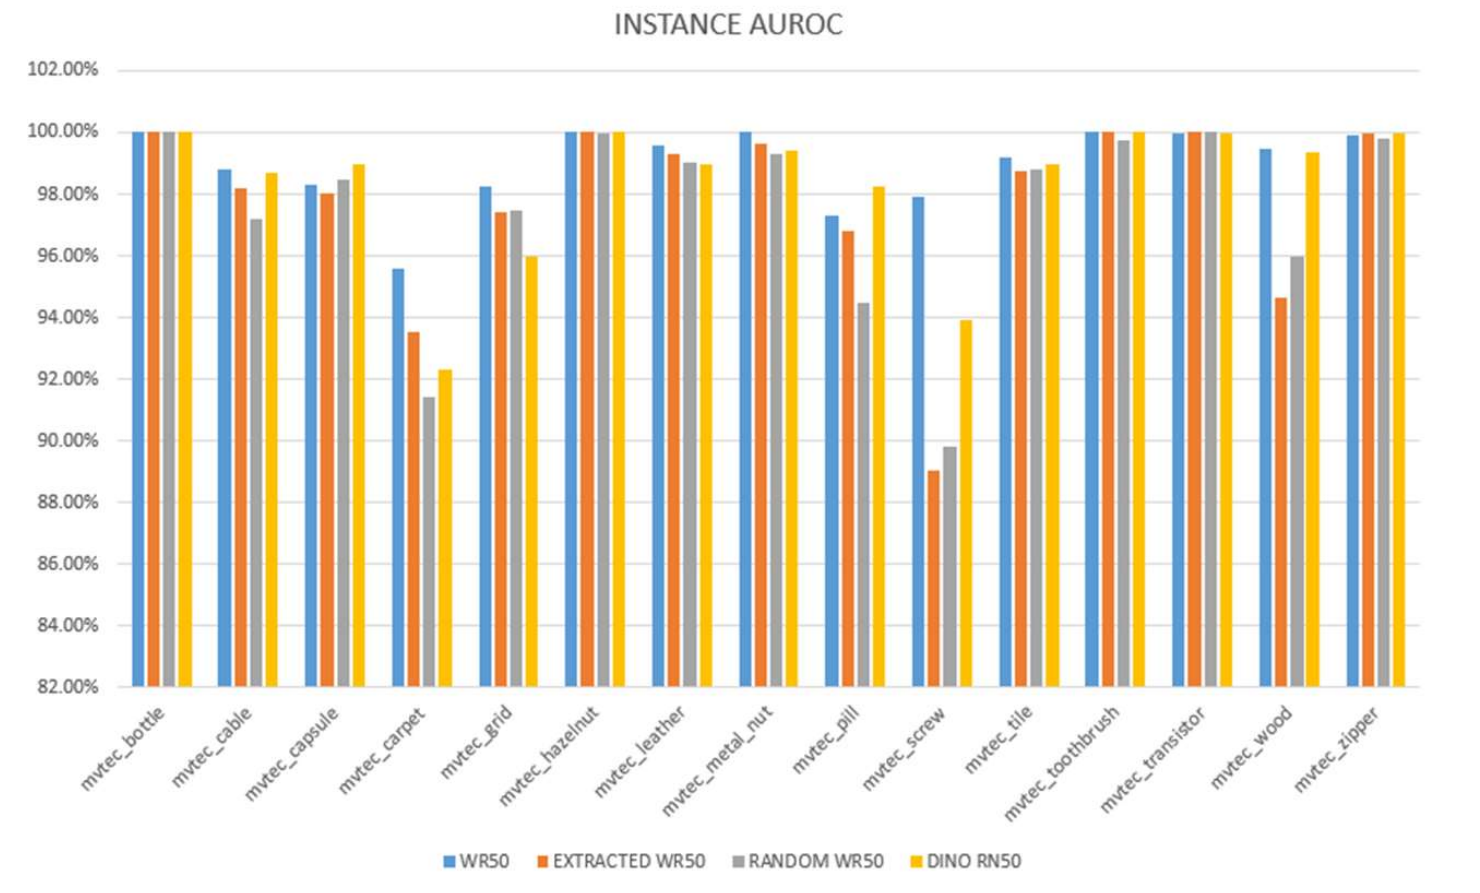
\includegraphics[width=1.0\linewidth]{Chapter_4/wd_instance.png}
	\end{center}
	\caption{Mean scores Instance AUROC, Full Pixel AUROC and Anomaly Pixel AUROC across all categories of MVTechAd dataset}
	\label{fig:wd_instance}
\end{figure}

\begin{figure}[h]
	\begin{center}
		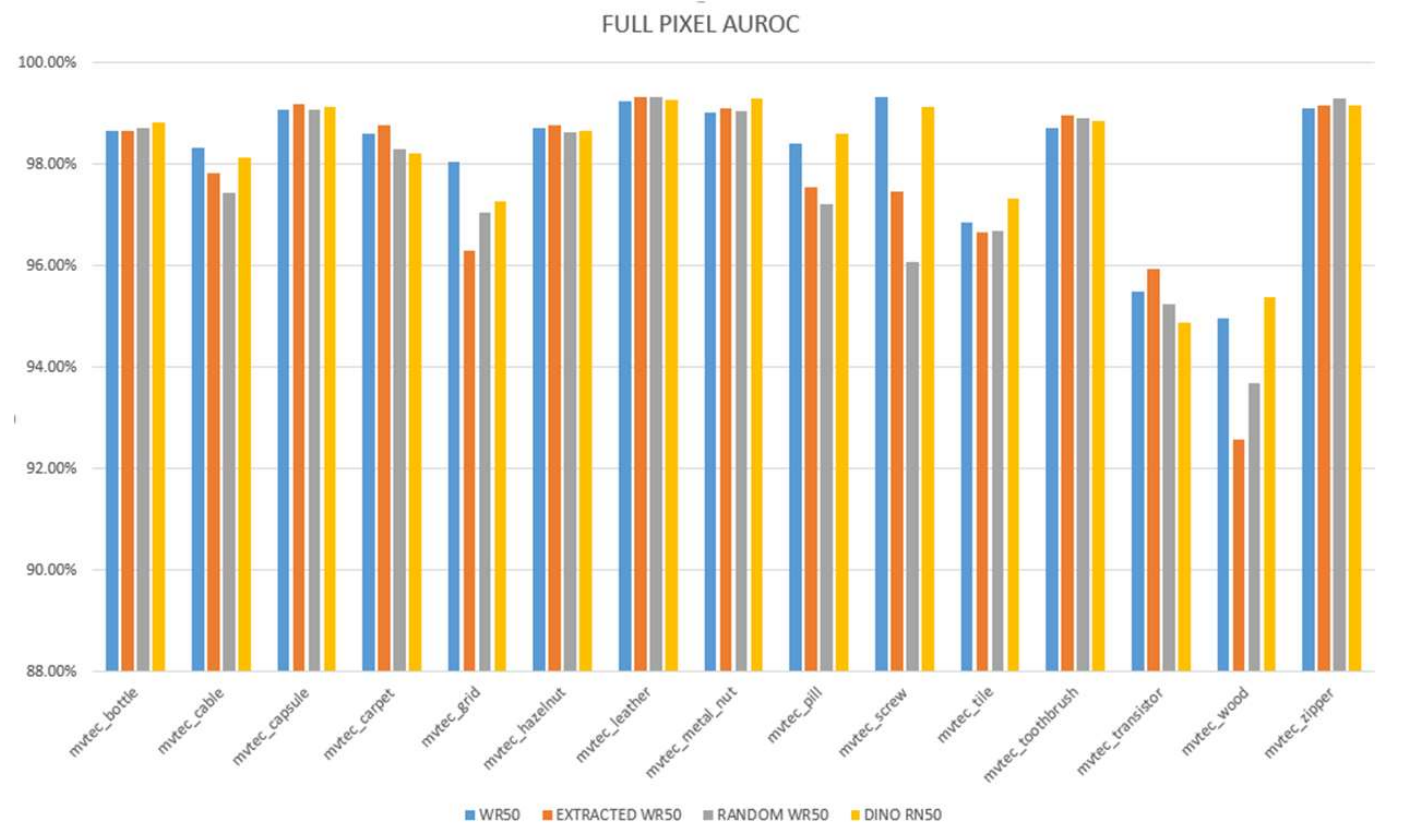
\includegraphics[width=1.0\linewidth]{Chapter_4/wd_full_pixel.png}
	\end{center}
	\caption{Mean scores Instance AUROC, Full Pixel AUROC and Anomaly Pixel AUROC across all categories of MVTechAd dataset}
	\label{fig:wd_full_pixel}
\end{figure}

\begin{figure}[h]
	\begin{center}
		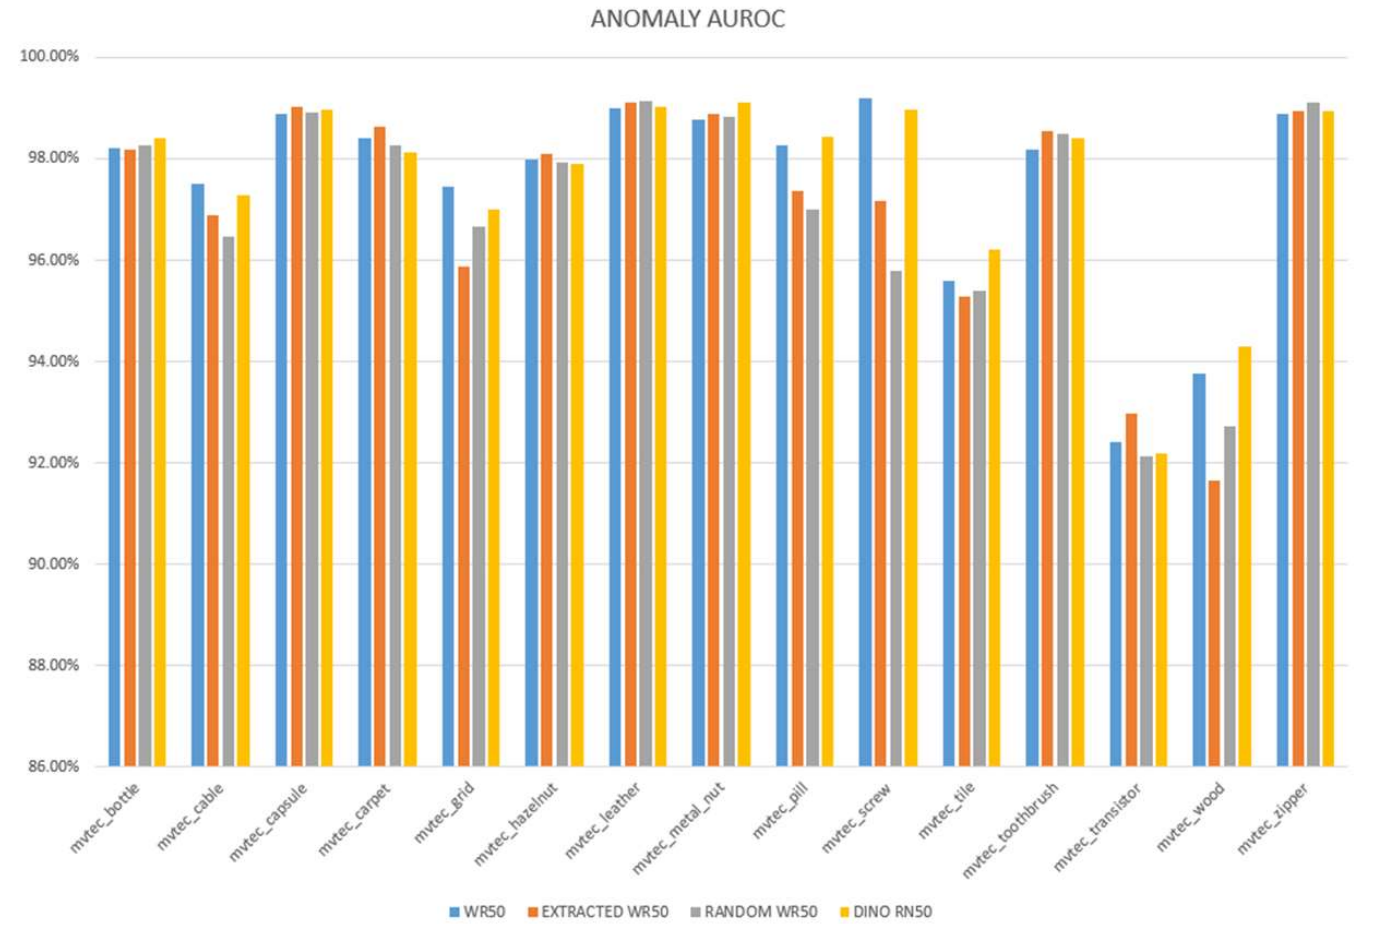
\includegraphics[width=1.0\linewidth]{Chapter_4/wd_anomaly.png}
	\end{center}
	\caption{Mean scores Instance AUROC, Full Pixel AUROC and Anomaly Pixel AUROC across all categories of MVTechAd dataset}
	\label{fig:wd_anomaly}
\end{figure}

\begin{figure}[h]
	\begin{center}
		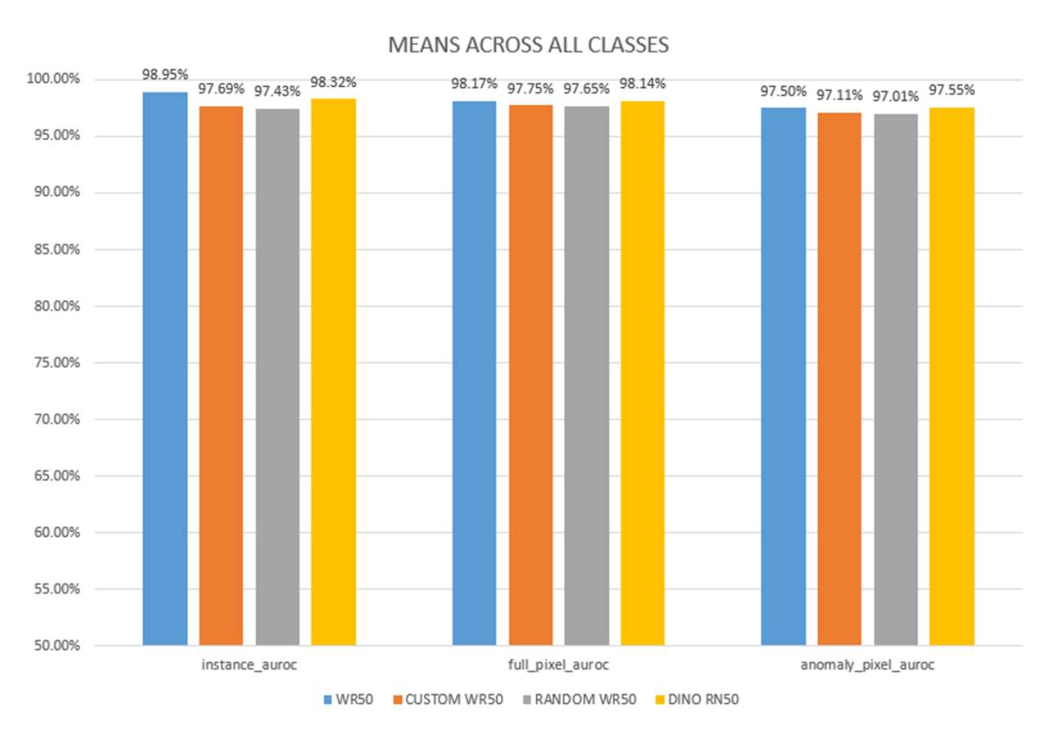
\includegraphics[width=1.0\linewidth]{Chapter_4/wd_mean.png}
	\end{center}
	\caption{Mean scores Instance AUROC, Full Pixel AUROC and Anomaly Pixel AUROC across all categories of MVTechAd dataset}
	\label{fig:wd_mean}
\end{figure}

\section{Selective extraction with LLM and VLM}

%%
%%% Chapter 5
\cleardoublepage
% \thispagestyle{empty}
% \mbox{}
% \newpage
\chapter{Conclusions and Future Improvements}
\label{chapter:ch5}

\section{Conclusions}

This thesis focused on the analyzing the usage of pre-trained feature extractors in industrial anomaly detection\cite{iad_survey}\cite{uiad_survey}\cite{pre_trained_iad} and possibly ways of improving the accuracy of models by addressing the hypothesized bottleneck. We postulated that the generality of ImageNet dataset\cite{imagenet}, on which most predominantly utilized pre-trained extractors trained on, could generate non-ideal features for the use in industrial settings. The postulation was motivated by the fact that ImageNet, in the considerable amount, consists of images that do not represent the industrial field nor do they relate to images that are commonly used in industrial tasks like MVTechAD\cite{mvtecad}. 

We presented two methods for addressing the proposed issue: selective image extraction by using a CNN\cite{lenet} bi-class classifier, selecteive image extraction with the help of Large Language Models(LLM)\cite{llm_survey}\cite{gpt3} and Vision Language Models(VLM)\cite{vlm_survey}\cite{clip}. First method relies on bi-class CNN model that was trained on pre-constructed dataset with labels "industrial" and "non-industrial". Second method is based on the generation of descriptors using an LLM and filtering images by a CLIP\cite{clip} cosine similarity score between the descriptors and samples. Both methods were applied to a large multi purpose dataset in order to generate a specialized dataset for industrial tasks. Throughout the work in this thesis both supervised and self-supervised learning methods\cite{self_supervised_survey}\cite{dino} were engaged to achieve feature learning.

After extensive series of experiments on the feature learned from extracted datasets, it was determined that the feature space of WideResNet\cite{wideresnet}, which is commonly used in contemporary industrial anomaly detection models\cite{patchcore}\cite{pre_trained_iad}, is surprisingly efficient and extremely resilient to scrutiny. Althoug we were successful in improving the performance in some categories of objects in the dataset MVTechAD, all attempts to outperform the state of the art pre-trained feature extractor in all categories were met with failure. However, we learned that the contents of the dataset from which features are learned from is very important.

In conclusion, through experiments we determined that ImageNet based feature spaces are surprisingly efficient for industrial anomaly detection tasks, despite the general nature of ImageNet dataset. Performance increase through improved feature space could still be achievable, but methods presented in this were proven to be inefficient in this task.

\section{Future Improvements}

As was stated in the previous section, we were able to archive higher than sota accuracies in several categories while under performing on others. This discovery demonstrates the feasibility of achieving overhead on the performance of the sota feature extractor. As per the selective extraction, designing the extraction pipeline more meticulously might show a promising performance. Another method to achieve an extraction of a high quality industrial dataset might be the usage of LLMs on large scale, CLIP labeled datasets like LAION5B\cite{laion5b}. For the dataset extraction methods, in our opinion, these seem to be the all possible options as of now.

For the feature space based improvements of industrial anomaly detection models, an approach used in the IAD model RealNet\cite{realnet} could be extended and utilized as a component in pipeline of other models. The approach is the feature selection during training time which consists of building a large scale general feature space with high variety in the features, and performing the selection of features that are best for the specific use case during training time\cite{realnet}. However, development as testing of such hypothesis might prove to be both very time and cost inefficient.

Lastly, introduction of anomalous features into a features space during pre-training as as the IAD models GLASS\cite{glass} and RealNet\cite{realnet} do during train time, could bring performance improvements. This could be achieved fine-tuning of the pre-trained feature extractor with artificially generated anomalies.

We believe that all the presented methods pose a potential for an improvement and needs further extensive investigation.


%
%%%%%% bibliography %%%%%%%%%%%%%%%%%%%%
%
\cleardoublepage
% \thispagestyle{empty}
% \mbox{}
% \newpage
\bibliographystyle{unsrt}
\bibliography{References/references}

%
%%%%%%% appendix %%%%%%%%%%%%%%%%%%%%%%%%
%
% \cleardoublepage
% \include{Publications/list_of_pubs}

%%%%%%%%%%%%%%% Acknowledgments %%%%%%%%%%%%%%%
%
\cleardoublepage
% \thispagestyle{empty}
% \mbox{}
% \newpage
% Acknowledgments.tex

\begin{acknowledgments}

First and foremost, I express my deep gratitude to my supervisor Professor Takayuki OKATANI for the immense support and illuminating guidance. Truly, without his guidance and unwavering will to share knowledge, this work would not be possible in the state that it is now. I am forever grateful for having the opportunity to work under his supervision.

I am deeply grateful to Professor Hiroyuki TAKIZAWA and Associate Professor Shingo KAGAMI for their invaluable contributions as members of my thesis committee. I am sincerely thankful for their time, support, and valuable input throughout the process.

I am sincerely grateful to Assistant Professor Masanori SUGANUMA for the guidance and encouragement during times of uncertainty an overall my research.

I would like to share my thankfulness to the members of the Computer Vision lab, namely Kang Jun LIU, Nguyen Van QUANG, Bonappol LIMANOND, Kitto?? for the support and experience they shared with me throughout my research. 

I also extend my appreciation for my family members, my parents BOBOJANOVA U. and BOLTABOYEV Sh. for their tremendous support throughout my life, without them I would not be here to write this work. I am also grateful to my sister RAKHIMOVA M. for always being encouraging and inspiring in all she does.

I am deeply appreciative of all the individuals mentioned above, along with everyone who, through various means, both directly and indirectly, have aided me in the completion of this work.

\end{acknowledgments}
%
%\cleardoublepage
\end{document}